\documentclass[a4paper, 11pt]{article}
\usepackage{graphicx}
\graphicspath{ {./images/} }
\usepackage{hyperref}
\hypersetup{
    colorlinks=true,
    linkcolor=blue,
    filecolor=magenta,      
    urlcolor=cyan,
}
\usepackage{listings}
\usepackage{xcolor}

\definecolor{codegreen}{rgb}{0,0.6,0}
\definecolor{codegray}{rgb}{0.5,0.5,0.5}
\definecolor{codepurple}{rgb}{0.58,0,0.82}
\definecolor{backcolour}{rgb}{0.95,0.95,0.92}

\lstdefinestyle{pythonstyle}{
    backgroundcolor=\color{backcolour},   
    commentstyle=\color{codegreen},
    keywordstyle=\color{magenta},
    numberstyle=\tiny\color{codegray},
    stringstyle=\color{codepurple},
    basicstyle=\ttfamily\footnotesize,
    breakatwhitespace=false,         
    breaklines=true,                 
    captionpos=b,                    
    keepspaces=true,                 
    numbers=left,                    
    numbersep=5pt,                  
    showspaces=false,                
    showstringspaces=false,
    showtabs=false,                  
    tabsize=2
}

\lstset{style=pythonstyle}
% define the title
\author{Nguyen The Minh}
\title{Computer Networking: The TCP/IP Architecture}
\begin{document}
% generates the title
\maketitle
\tableofcontents
\newpage
\section{Introduction to Computer Network}

To study computer networking, we will explore the public Internet that is a specific global computer network. And to understand the Internet, we will describe basic hardware and software components that make up the Internet. We also describe the Internet in term of a networking infrastructure that provides services to distributed applications.\\

Basically, a computer network is a collection of computers. They communicate to each other to form a network. The term computers are general, they maybe various devices such as PC, laptop, server computers, smartphone, TV, car, sensors, and many many other embedded devices.\\

Internet is the global computer network. There are billions of devices in Internet.\\

Internet is very huge. Of cause, nobody or no organization can manage it alone. Internet is constructed recursively and composed of smaller parts. Therefore, the network is a recursive term. Some networks are connected together to form a bigger network - \textbf{internetwork}. Small networks are built and managed by individual organizations.\\

We can think about a computer network as a graph. In there, nodes are devices and edges are physical links (wire or wireless links) between these devices.\\

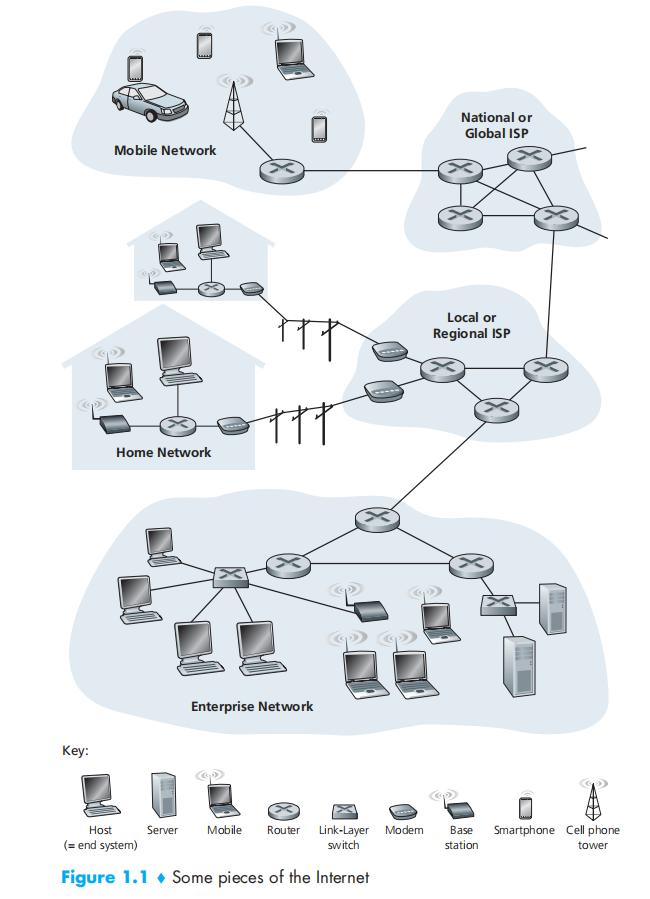
\includegraphics[width=12cm]{pieces-of-internet.png}\\

Two computers can communicate or exchange data through many physical channels and technologies:\\
\begin{itemize}
\item Wire channels: twisted pair cable, coaxial cable, optical fiber
\item Wireless channels: WiFi, Bluetooth, Zigbee, Satellite
\end{itemize}

Each technology has a different way to transmission data and different bandwidth.\\

Bandwidth is the capacity of data exchange and measured by bits/s. For example, an Ethernet-link has bandwidth of 100Mb/s, 1Gb/s, to 10Gb/s. WiFi-link has the less bandwidth, from 10Mb/s to 1Gb/s. Don't confuse with bandwidth term in the electrical engineering that is measured in Hz to tell how width of signal frequency range supported by a specific channel.\\

\clearpage
\section{Network characters}

\textbf{Network size}\\
Local area network (LAN) is a network of computers typically inside a building like a home or an office. LANs are basic elements of the Internet, we will talk about they later deeply.\\

Wide area network (WAN) is a network that extends over a large geographic such as a city, a region. Global network or Internet is a network of the world.\\

\noindent \textbf{Wire and wireless}\\
Computers can connect together using wire or wireless links.\\
Wire links use electrical signal through copper cable or optical signal (laser or LED) to transmission data.\\
Wireless links use radio signal to transmission data.\\

\noindent \textbf{Circuit and Packet switch}\\
In a circuit switching network, before each communication session, a dedicated path through two devices is established and some bandwidth is saved and exists during the session and free at the end of the session. The circuit network (e.g, Telephone network) guarantees the quality of service (not interrupted, stable throughput). In a packet switching network, data are sent through network packet by packet, hop by hop, no guarantee of the quality of service.\\

Circuit switching networks guarantee the quality of service but more expensive than packet switching networks. And total throughput in a packet switching network will be much more than a circuit one.The Internet is designed as a packet switching network.\\

In a connection-oriented communication, a logical connection must be established between two devices before they exchange data. Connectionless fashion doesn't establish a connection between devices. As soon as a device want to send data, it just sends it.\\

Circuit-switched networks are inherently based on connections. While in packet-switched networks, connections can be logical created, but are optional. We'll explore the TCP protocol as a connection-oriented protocol later.\\

\clearpage
\section{Network services and layered architecture}

A computer want to exchange data with another, it must know how to address its participant and how to send data through different links. There are many physical link types: wire and wireless; copper cable and optical fiber;  WiFi, Bluetooth and Satellite; GSM, 3G and 4G. And communication is direct or indirect. Direct means two computers are connected by a physical link directly. Indirect means two computers are connected by series of physical links. Two computers are connected by a direct link is same as two adjacent nodes in a graph.\\

Besides the addressing issue, computer networks have to support transmitting data effectively. The Internet is a huge and dynamic computer network. Devices and links are added or removed anywhere and anytime. It needs a routing solution to find paths to transmit data effectively in some balanced manners.\\

Data was exchanged must be correct. As we know, data were divided into many packets and they were transmitted one by one through the network from a device to another. Data transmission needs the integrity property, that means packets received by the receiver must be the same as packets that were sent by the sender. Networking must have the ability to detect error packets, and tell end devices these errors or maybe correct them. In addition, a network could provide a reliable delivery service. Internet services could guarantee that packets will be sent to the receiver, and/or in the correct order. And there are some services that Internet could provide. We'll explore them in particular sections.\\

To address the complex networking problem, the Internet was designed as a layered architecture. Each layer will solve a facet of the networking problem. Layers communicate with those above and below via concise interfaces. This layered representation leads to the term protocol stack, which refers to the stack of layers in the protocol suite. The Internet uses the TCP/IP architecture or the TCP/IP protocol suite. \\

\begin{figure}[h]
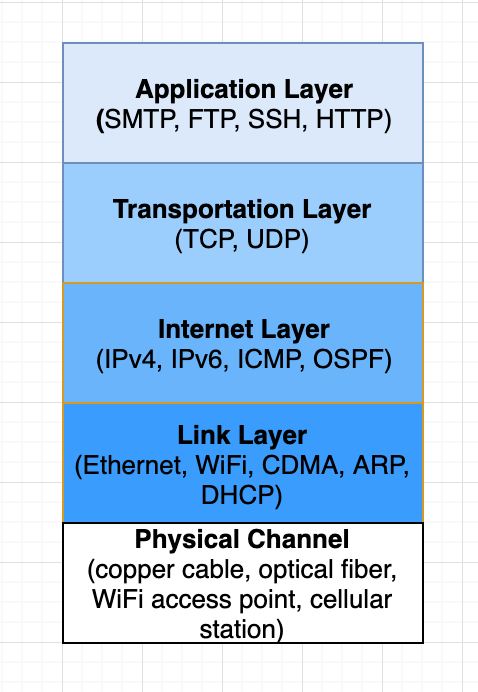
\includegraphics[scale=0.6]{networking-layers.png}
\end{figure}

Each layer will have a set of protocols to form the layer's service. A protocol is the way of data transmission. It defines the steps and message formats in order to communicate. All devices in the network have to follow these protocol to work together.\\

\textbf{Application Layer} defines application protocols that are used by any application programs. A application is a user process cooperating with another process usually on a different host. It uses the TCP/IP for communication. Examples of applications include Telnet, Web (HTTP), and File Transfer Protocol (FTP). The interface between the application and transport layer is sockets, which we will describe later and in more detail in another article.\\

\textbf{Transport Layer} provides end-to-end transfer by delivering data from an application to its remote peer. The most important transport protocol is the Transmission Control Protocol (TCP), which provides connection-oriented reliable data delivery, congestion control, and flow control. Another transport protocol is the User Datagram Protocol (UDP). It provides connectionless, unreliable, best-effort service. Usually, UDP is used by applications that need a fast transport mechanism and can tolerate the loss of some data.\\

\textbf{Internetwork Layer} or Network Layer provides a routing function to route data across the Internet - network of networks. Internet Protocol (IP) is a center protocol in this layer. It is connectionless, unreliable, no flow control, no error recovery protocol. These functions must be provided at a higher level. Other internetwork-layer protocols are ICMP, IGMP, ARP, and RARP.\\

\textbf{Link Layer} or data-link or network interface layer, is the interface to actual network hardware. There are many protocols in this layer. Examples are Ethernet, WiFi, X.25, ATM, FDDI. TCP/IP specifications don't describe or standardize any link-layer protocols, they only standardize the ways of accessing those protocols from the internetwork-layer.\\

When receiving a data unit (packet, message, ..), called \textit{a protocol data unit (PDU)} from a higher layer, the current layer will encapsulate the data unit by adding some header and/or some trailer (footer) fields to create a new data unit. In the Transport Layer, PDU has a name called \textit{segment}, \textit{datagram} in the Internetwork layer, and \textbf{frame} in the Link layer.

\begin{figure}[h]
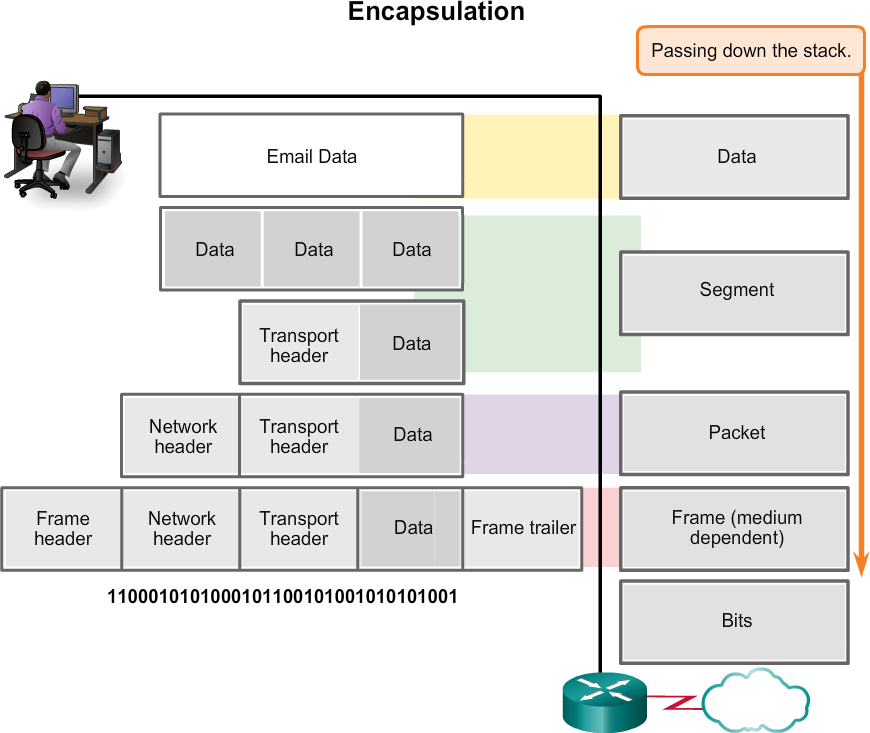
\includegraphics[scale=0.5]{protocol-data-unit.png}
\caption{Data encapsulation and protocol data unit at each layer}
\end{figure}

\clearpage
\section{Link Layer}

\begin{figure}[h]
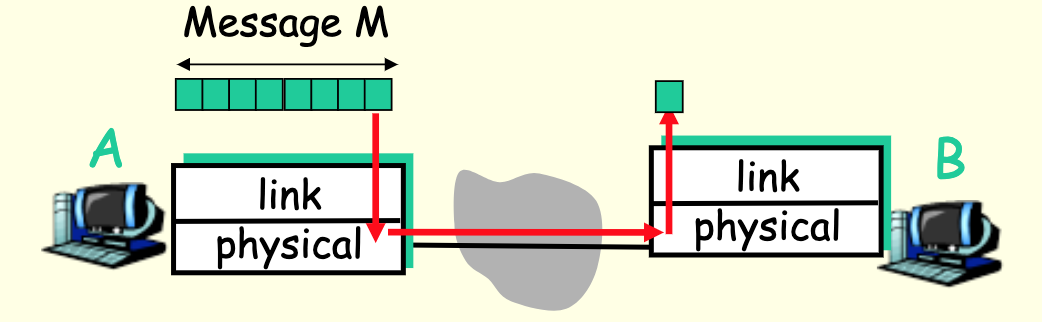
\includegraphics[scale=0.5]{link-layer.png}
\caption{Link layer: How computer talk to its neighbor}
\end{figure}

Link layer has responsibility of transferring data packets (datagram) from the internetwork layer from one node to \textbf{physically adjacent} node over a link. \\

\begin{itemize}
\item \textbf{Link} can be \textit{guided} media(a copper, coax, fiber wire) or \textit{unguided} media(wireless)
\item \textbf{Link} can be \textit{point-to-point} or \textit{broadcast} (shared links)
\end{itemize}

There are possible services the link layer can support:\\

\begin{itemize}
\item \textbf{Framing}. Detecting frame boundaries by encapsulating datagrams (data packets from the internetwork layer) in to frames, adding headers, trailers
\item \textbf{Link access}. When a link is shared by many devices, to determine which device can use the link to the problem need to solve. There are some protocols related to different technologies of the link layer will address this problem.
\item \textbf{Reliable delivery}. The high error rate links often provide a reliable delivery service to correct errors locally rather than end-to-end retransmission of the data from higher layers.
\item \textbf{Error detection and correction}. A bit was transmitted can be flipped from 0 to 1 and vice versa. These errors can be introduced by signal attenuation or electromagnetic noise. Link layer protocols provide a mechanism to detect and/or correct these errors. Error detection usually is implemented in hardware. Other errors maybe detect and correct in higher layer protocols.
\end{itemize}

In a broadcast link, how a computer tell that the frame is sent to which other? It is addressing problem. Each node MUST have an unique address, called the Media Access Protocol address or MAC address. The MAC address is the 48-bit, usually persistent, flat address, no hierarchical organization, and space managed by IEEE. When framing, the link layer attaches source and destination MAC address into the frame header.

The link layer is implemented in a \textbf{network interface card} (NIC), also known as \textbf{network adapter}. The network adapter contains a controller, which called link layer controller, a special-purpose chip that implements many link layer services (framing, link access, error detection, and so on). For example, Intel’s 8254x controller implements the Ethernet protocols, the Atheros AR5006 controller implements the 802.11 WiFi protocols. \\

\begin{figure}[h]
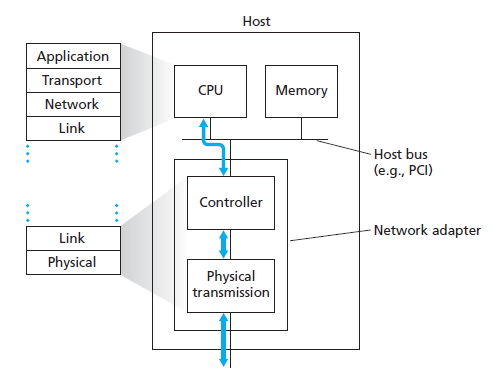
\includegraphics[scale=0.8]{network-adapter.png}
\caption{Network adapter}
\end{figure}

Network adapters are attached to host's system buses. They look like any other I/O device to the host. Host's software will respond to controller interrupts(e.g., due to receipt of one or more frames), passing datagrams to the internetwork layer.

\subsection{Ethernet}

We'll cover the most popular link-layer protocol called Ethernet. The term Ethernet generally refers to a set of standards used to build LAN networks. The first Ethernet standard called \textit{shared Ethernet}, and it was adopted by the IEEE as standard number 802.3. A shared Ethernet network will be arranged as the following figure.\\

\begin{figure}[h]
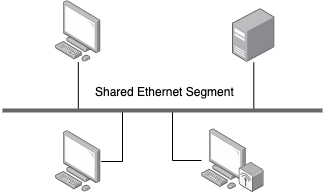
\includegraphics[scale=0.6]{shared-ethernet.png}
\caption{A shared Ethernet network consists some devices (stations) attached to a shared cable segment}
\end{figure}

Because multiple stations shared the same medium link, a distributed algorithm will be implemented in each Ethernet network interface that controls when a station gets to send data it has. Some protocols has developed called Media Access Protocols (MAC protocols) to solve this problem. The particular method, known as \textit{carrier sense, multiple access with collision detection} (CSMA/CD), meditates which computers can access the shared medium link.\\

Other Ethernet network type is switched Ethernet, which is more popular today. A switched Ethernet network is formed by a \textbf{switch} and many stations connect to a port of the switch directly. There are no shared medium link. In most case where switched Ethernet is used, the network operates in a full-duplex fashion (sending and receiving simultaneously) and the CSMA/CD algorithm is unnecessary.\\

\begin{figure}[h]
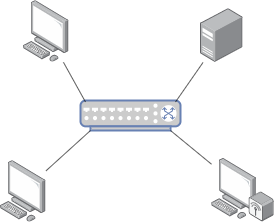
\includegraphics[scale=0.6]{switched-ethernet.png}
\caption{A switched Ethernet network consists a switch and many stations, each of which is attached to a switch port using a separated link}
\end{figure}

Two switched Ethernet networks can combine together by switch ports to build a larger switched Ethernet network.\\

\begin{figure}[h]
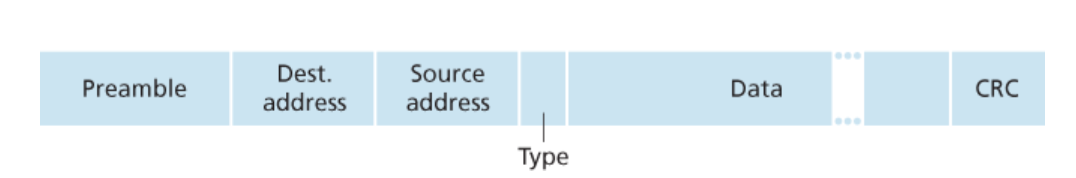
\includegraphics[scale=0.6]{ethernet-frame-format.png}
\caption{A Ethernet Frame Format}
\end{figure}

To learn more about Ethernet, we will explore the format of a Ethernet frame. Let the sending adapter, adapter A, has the MAC address AA-AA-AA-AA-AA-AA and the receiver, adapter B, has the MAC address BB-BB-BB-BB-BB-BB.\\

\begin{itemize}
\item \textbf{Preamble (8 bytes).} Each of the first 7 bytes of the preamble has a value of 10101010; the last byte is 10101011. The first 7 bytes of the
preamble serve to “wake up” the receiving adapters and to synchronize their clocks to that of the sender’s clock. 
\item \textbf{Destination address (6 bytes).} This field contains the MAC address of the destination adapter, BB- BB-BB-BB-BB-BB. When adapter B receives an Ethernet frame whose destination address is either
BB-BB-BB-BB-BB-BB or the MAC broadcast address (FF-FF-FF-FF-FF-FF), it passes the contents of the frame’s data field to the network layer; otherwise, it discards the frame.
\item \textbf{Source address (6 bytes).} This field is the MAC address of the sender, adapter A, is AA-AA-AA-AA-AA-AA.
\item \textbf{Type field (2 bytes).} Indicating which network-layer protocol using (e.g., IP, IPX or ARP protocol).
\item \textbf{Data field (46 to 1500 bytes).} This field carries the network-layer datagram. The maximum transmission unit (MTU) of Ethernet is 1500 bytes. If the datagram exceeds 1500 bytes, the host has to fragment the datagram. If the datagram is less than 46 bytes, the host has to fit it to 46 bytes by "stuffed". The network layer uses the length field in the datagram header to remove the stuffing.
\item \textbf{Cyclic redundancy check (CRC) field.} The value of the CRC algorithm used to detect errors in the frame.
\end{itemize}

\subsection{Bridges and Switches}

A bridge or switch is used to join some physical link-layer networks (e.g., a pair of Ethernet segments). An example is connecting two switches to form a extended LAN, as shown in the figure~\ref{fig:extend-LAN}.

\begin{figure}[h]
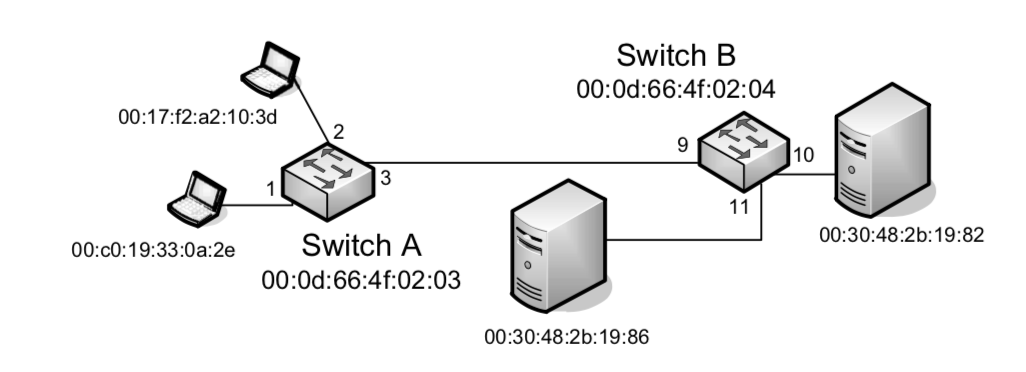
\includegraphics[scale=0.6]{extended-LAN.png}
\caption{A extended Ethernet LAN with two switches. Each switch port has a number for reference. Each stations, include switches, has a MAC address}
\label{fig:extend-LAN}
\end{figure}

The switch will learn MAC addresses of stations in the LAN network to know how to forward data (sent to it) to which port for efficient instead of flooding data to all ports. Learned MAC addresses with ports will be save in the switch's database like the figure~\ref{fig:switch-database}

\begin{figure}[h]
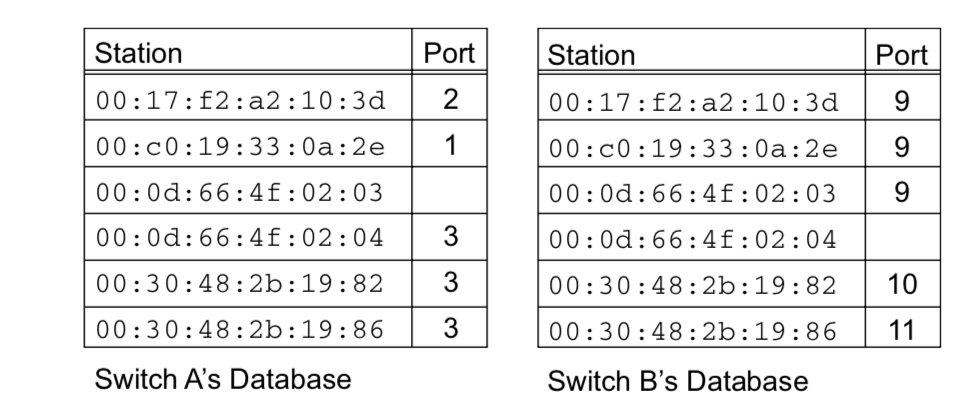
\includegraphics[scale=0.6]{switch-database.png}
\caption{Switch filtering databases are created and updated over time(learned) by the observing source address on frames seen on ports}
\label{fig:switch-database}
\end{figure}

When a switch is first turned on, its database is empty, so it doesn't know the address of any station. Wherever it received a frame, it saves the source address from the frame and the port, which the frame come to, into its database. This is the way switches learn the location of all stations in the LAN network. If the switch received a frame with the destination address it hasn't known, it will flood the frame to all ports except the port the frame arrived, else it forward the frame to only port that has the same attached MAC address with the destination address.\\

\subsection{WiFi and the IEEE 802.11 Wireless LAN}

In a WiFi network (802.11 Wireless LAN), all hosts connect to a center device called \textbf{Access Point} (same purpose as a Ethernet switch) through wireless links - communication by radio signals. Hosts can communicate to each other or to external hosts via the Access Point. All these hosts are called wireless hosts. They might be a laptop, tablet, smartphone, or desktop computer.\\

\begin{figure}[h]
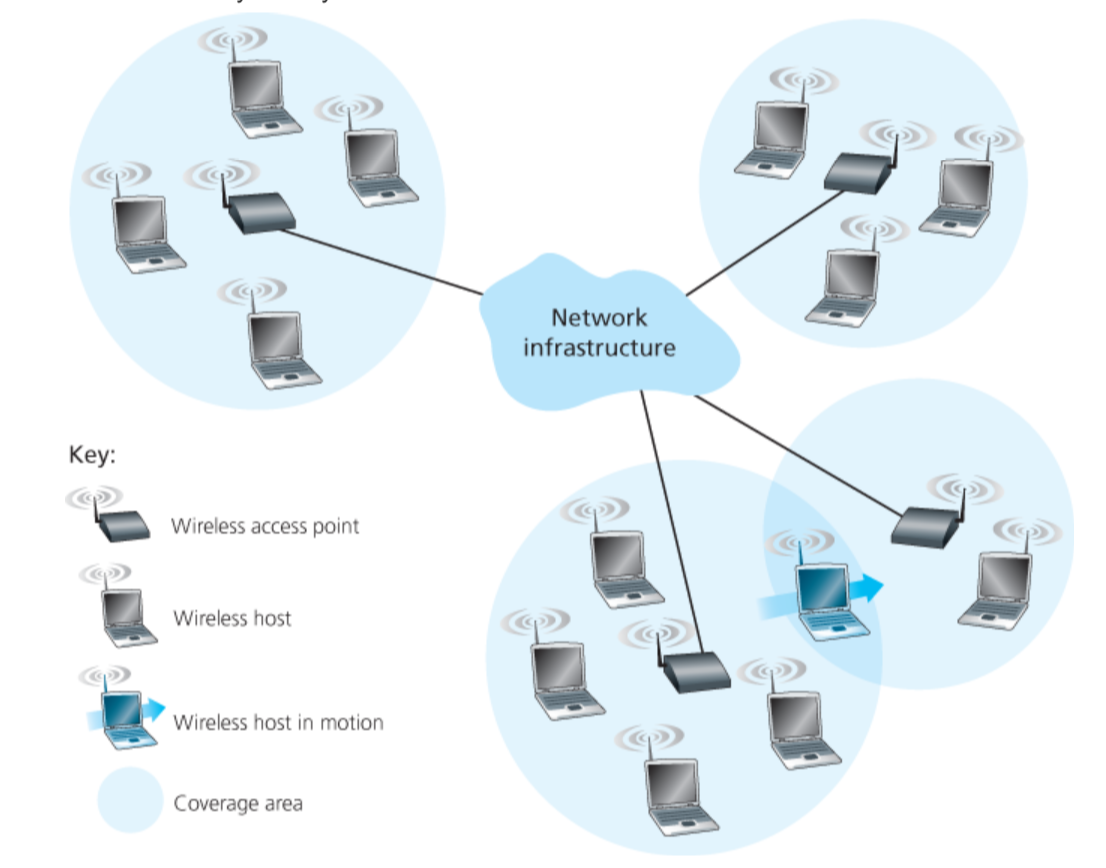
\includegraphics[scale=0.6]{wireless-network.png}
\caption{Wireless network elements}
\label{fig:wireless-network}
\end{figure}

Wireless links have some major different characters to wired links:\\

\begin{itemize}
\item \textbf{Decreasing signal strength.} As the distance between sender and receiver increases, the signal strength will decrease, the signal might disperse (referred as \textit{path lost}). Radio signal may be attenuated when it passes through material like a wall.
\item \textbf{Interference from other source.} Signal interference occurs when there are more one signal source exist or there is electromagnetic noise within the environment(e.g., a nearby microwave). This interference can lead to information errors. That means receivers can receive incorrect radio signals.
\item \textbf{Multipath propagation.} In radio communication, \textit{multipath} is the result in that radio signals reaching the receiver by two or more paths cause by for example of \textit{reflection} from water and some object like buildings. Multipath propagation causes multipath interference.
\end{itemize} 

From these characters of wireless links, we can see that bit errors will be more common in wireless links than in wired links. For this reason, wireless link protocols (such as the 802.11 protocol) employ not only error detection codes CRC, but also link-layer reliable-data-transfer protocols that correct or re-transmit corrupted frames.\\

Wireless networks are broadcast communication as their nature. Radio signals are sent will propagate all through the area and can be catch by all devices.  Many devices may send data at the same time. Hence wireless networks need a Media Access Control (MAC) protocol. WiFi (the 802.11 wireless LAN) uses the CSMA/CA protocol as a MAC protocol.\\

Some wireless networks can compose together to establish an extended network. Let see the 802.11 wireless LAN architecture in the figure~\ref{fig:802.11-architecture}

\begin{figure}[h]
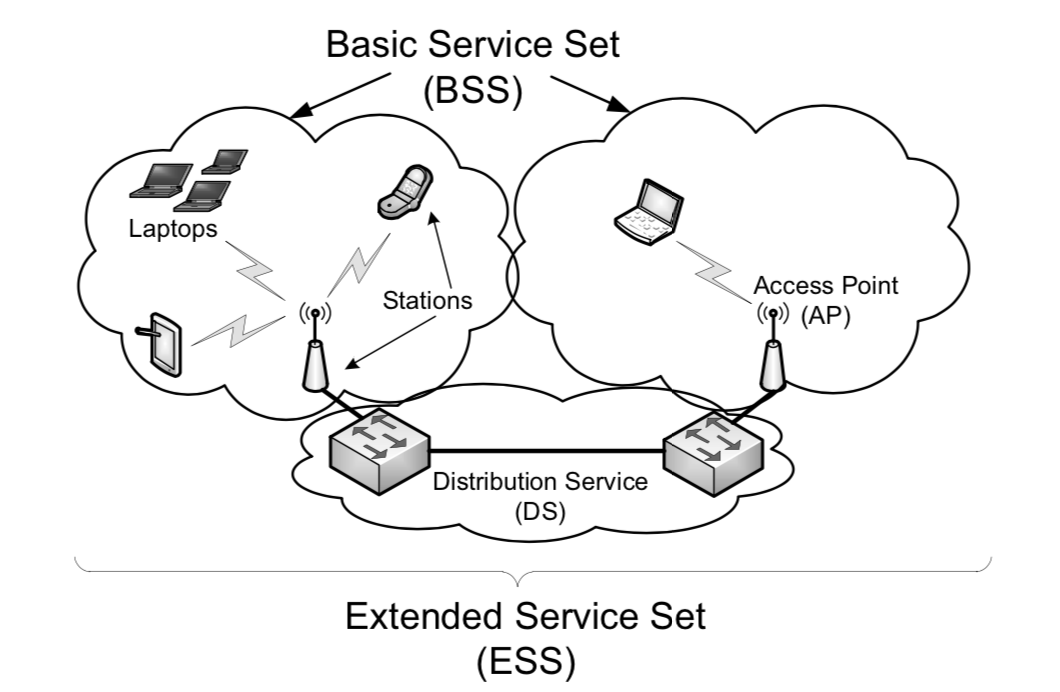
\includegraphics[scale=0.6]{80211-wireless-LAN-architecture.png}
\caption{IEEE 802.11 Wireless LAN architecture}
\label{fig:802.11-architecture}
\end{figure}

An Access Point(AP) and its associated devices (hosts) form a \textit{basic service set(BSS)}. Two APs are usually connected together using a wired \textit{distribution service(DS)}, forming an \textit{extended service set(ESS}. This setup called \textit{infrastructure mode}. In an \textit{ad hoc mode}, there is no AP or DS, hosts communications are direct peer-to-peer. A WLAN formed from a collection of BSSs called a \textit{service set}, identified by \textit{SSID} - typical 32 characters long is assigned to each AP by the network administrator.\\

Now, let examine the WiFi (802.11) frame format. The 802.11 frame format is similar to the Ethernet frame (studied above), but contains some fields that are specific to wireless links.\\

\begin{figure}[h]
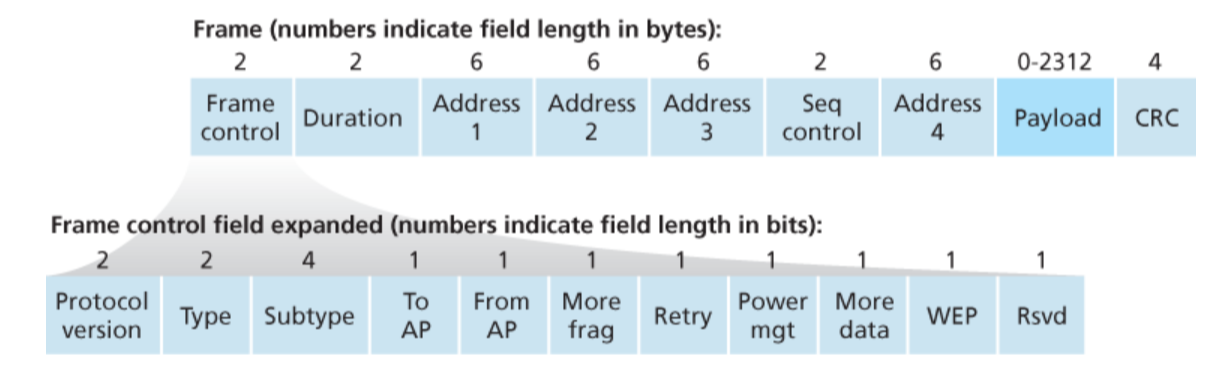
\includegraphics[scale=0.6]{80211-frame-format.png}
\caption{The 802.11 frame format}
\label{fig:802.11-frame-format}
\end{figure}

There are four MAC address fields: address 1 is the receiver, address 2 is sender, address 3 is used for filtering purposes by the receiver. Address 4 is only present in data frames transmitted between access points in an \textbf{Extended Service Set} or between intermediate hosts in a \textit{ad hoc network}.

To see more detail about MAC address, please visit \href{https://networkengineering.stackexchange.com/questions/25100/four-layer-2-addresses-in-802-11-frame-header}{MAC Addresses}.\\

\clearpage
\section{Internetwork Layer}

Recall that the Internet is a network of networks (internetwork) that are connected together using special devices called \textbf{routers}. Internetwork layer (Network layer) will solve the problem of delivering data between hosts, which lives across the Internet. To maximum the effectiveness of delivering, Internetwork layer have to implement a \textit{routing} algorithm to determine the best path to deliver a data unit (in particular is a segment from Transport Layer) between two end hosts. Figure~\ref{fig:network-layer} show a network with two hosts H1 and H2 and serveral routers on the path between them. At the sending side (H1), the network layer takes segments from the transport layer, encapsulates each segment into a datagram, and then sends the datagrams to its nearby router, R1. At the receiving host, H2, the network layer receives the datagrams from its nearby router R2, extracts the transport-layer segments, and delivers the segments up to the transport layer at H2. The routers path from R1 to R2 will be dynamically determined by a distributed routing algorithm of the network layer.\\

\begin{figure}[h]
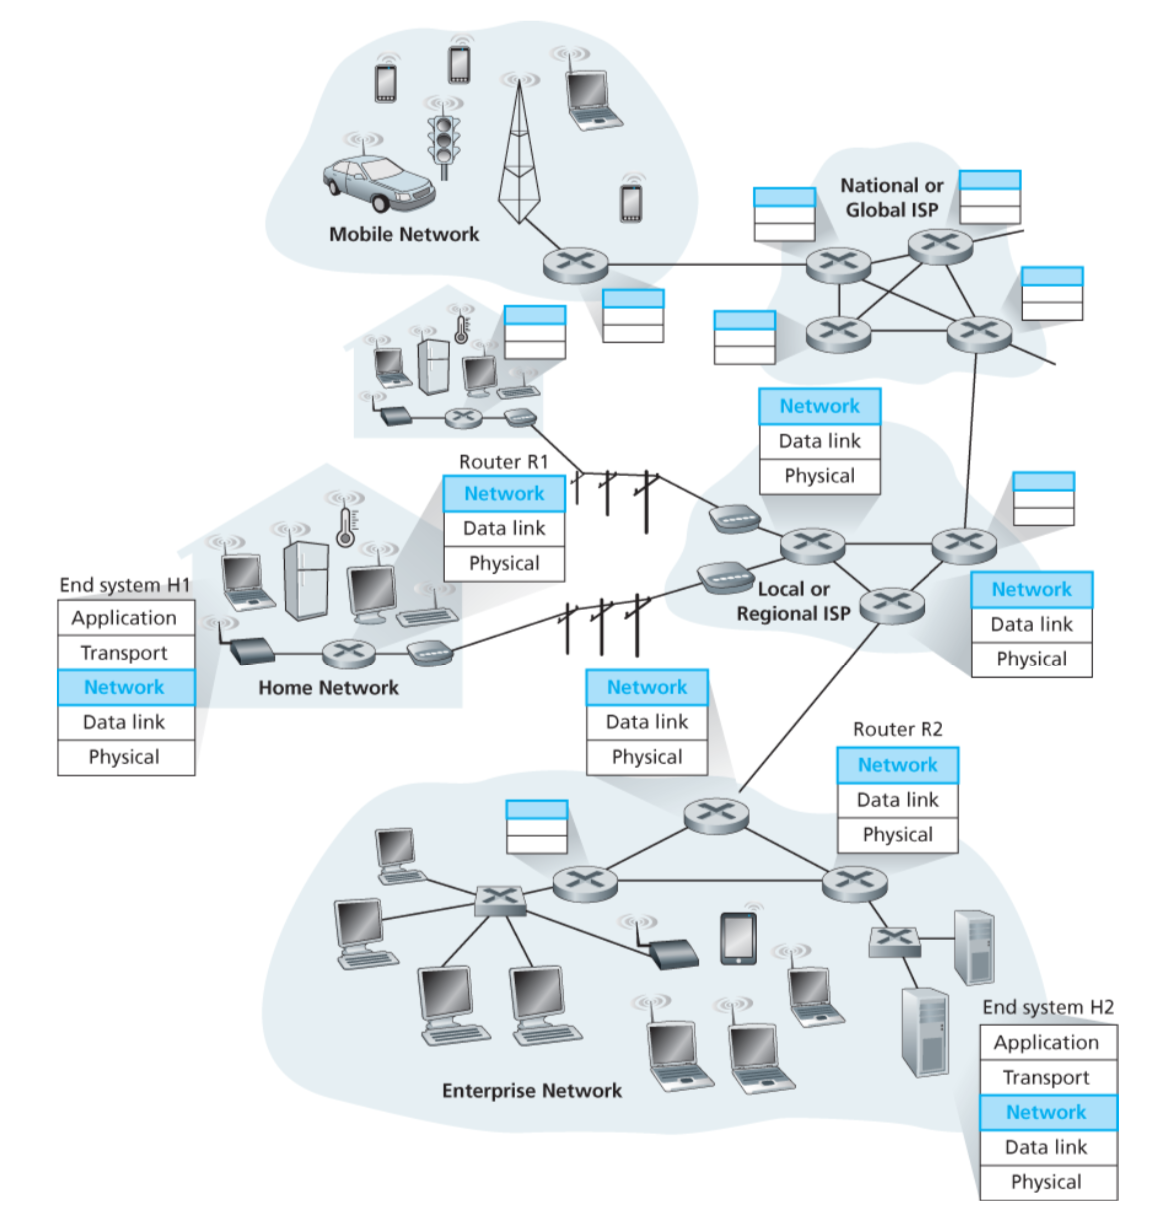
\includegraphics[scale=0.6]{network-layer.png}
\caption{The network layer}
\label{fig:network-layer}
\end{figure}

To implement the routing algorithm, Internetwork Layer defines a set of protocols and a logical addressing system. Every internetwork device will implement this set of protocol and every of them will has a unique address called an IP (Internet Protocol) address. 

\subsection{IP Addressing}

IPv4 (IP version 4) address is 32 bits wide. This provides theoretical \textit{address space} of $2^32$, or 4,294,967,296 addresses. IPv6 address is 128 bits wide, you see more about IPv6 in another reference. A IP address is usually represented as  dotted-decimal form. For example, the IP address 193.32.216.9. 193 is the decimal value of the first 8 bits of the address, 32 is the decimal value of the second 8 bits, and so on. The binary representation of this address is 11000001 00100000 11011000 00001001. Typically, a host has one link to the network. The data is sent over this physical link. The boundary between the host and the link is called an \textbf{interface}. A router's job is forwarding data, receive a datagram from one link and forward to another link. Therefore, a router have two or more links connected with it and it will have two or more interfaces.  In the Internet, each host or each interface has an unique IP address, accept behind NATs (discuss later in \ref{NAT}).\\

IP addresses are divided and manged as a hierarchical structure. The address space is divided into many small groups. Each of group can be divided into many smaller groups, and so on. This structure is called the \textbf{subnet} address architecture. The notation 223.1.1.0/24 means that 24 leftmost bits is the \textit{subnet ID or network prefix} and remaining bits is host ID. /24 is called \textit{subnet mask} that means using 24 leftmost bits as the subnet ID. 
A subnet mask can be written in the decimal form like 255.255.255.0 (there are 24 left most bits 1 in the binary representation).\\

\begin{figure}[h]
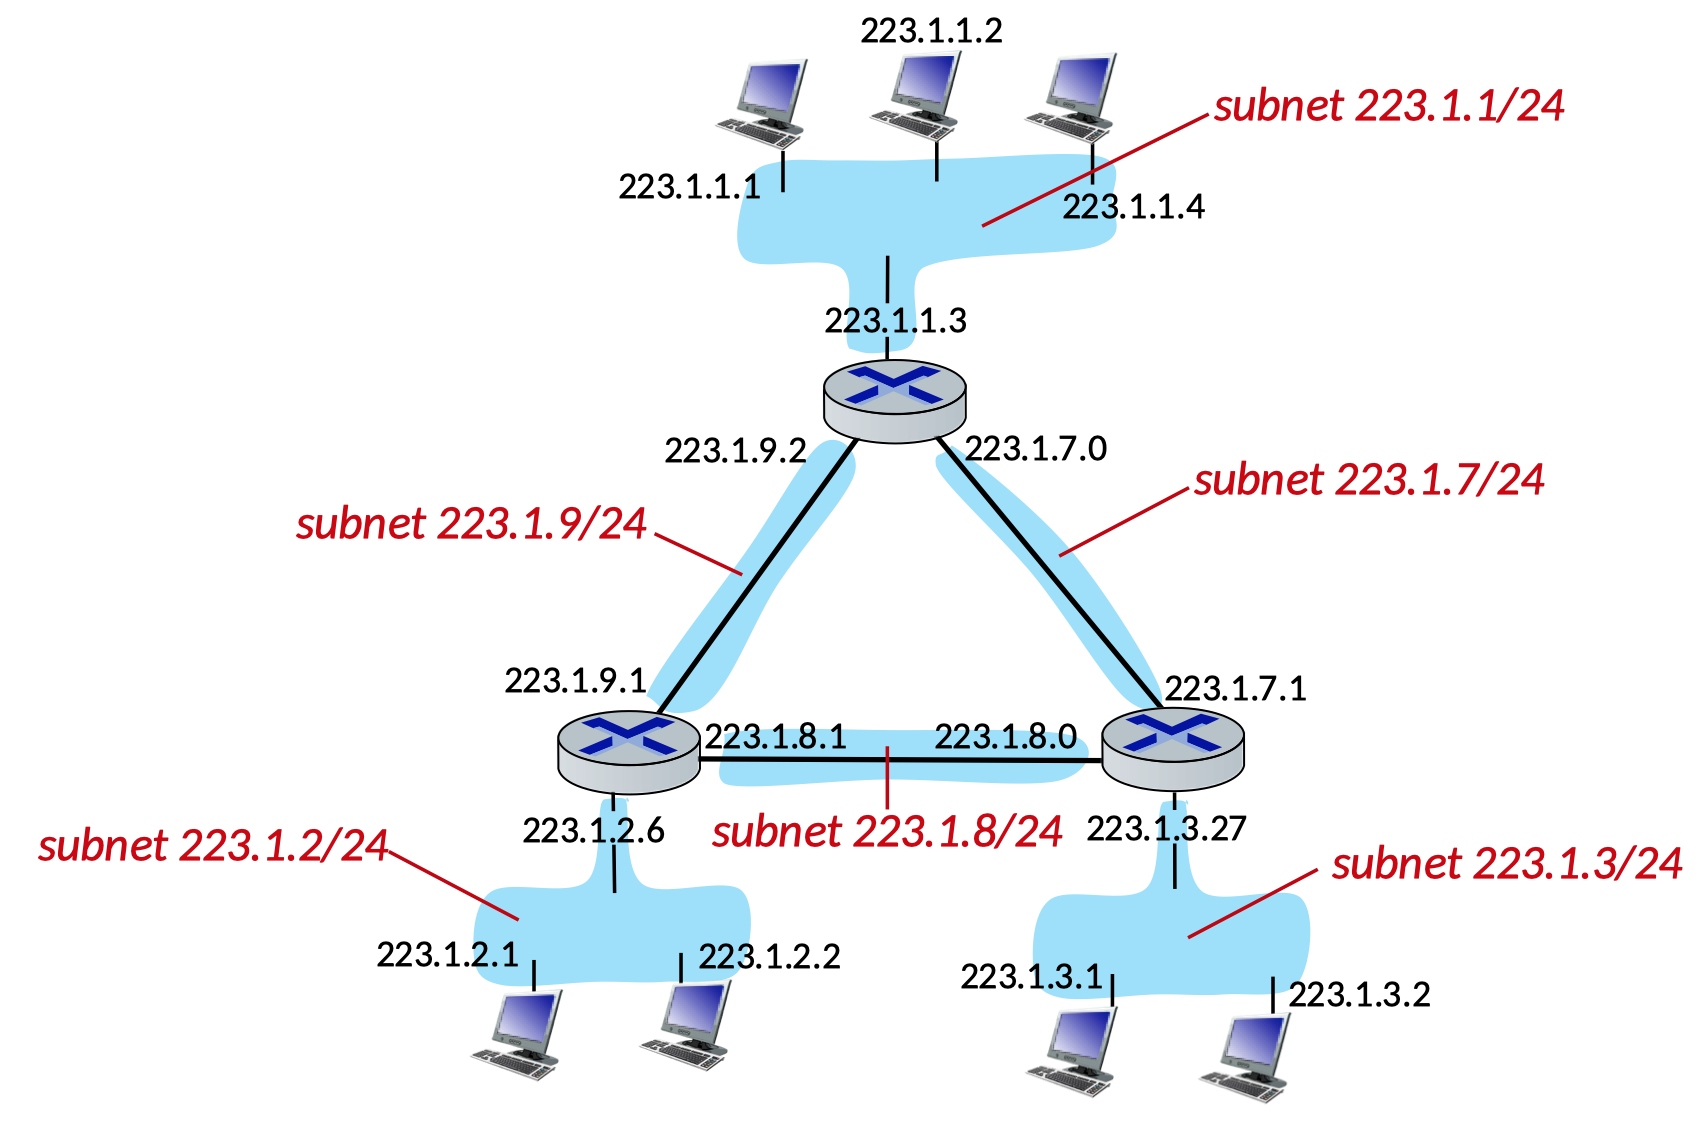
\includegraphics[scale=0.4]{subnet-example.png}
\caption{The subnet example}
\label{fig:subnet-example}
\end{figure}

There are some addresses are designed with a special purpose, shown in Figure~\ref{fig:special-ip-address}.\\

\begin{figure}[h]
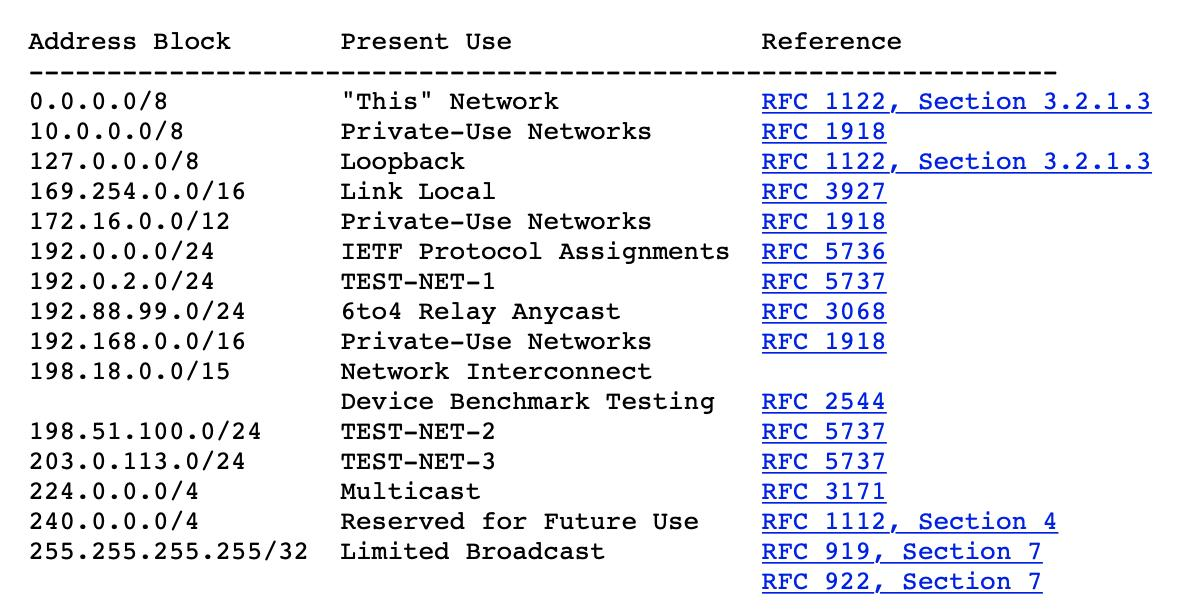
\includegraphics[scale=0.3]{special-ipv4.jpg}
\caption{Special use IPv4 addresses}
\label{fig:special-ip-address}
\end{figure}

\subsection{NAT-Network Address Translation} \label{NAT}

Many \textbf{private networks} such as  home networks, office networks can use the same \textit{private address space}, 10.0.0.0/8 address space is reversed for private networks, by using a technology called NAT - Network Address Translation that is implemented inside routers. We call these routers - NAT-enabled routers.\\

\begin{figure}[h]
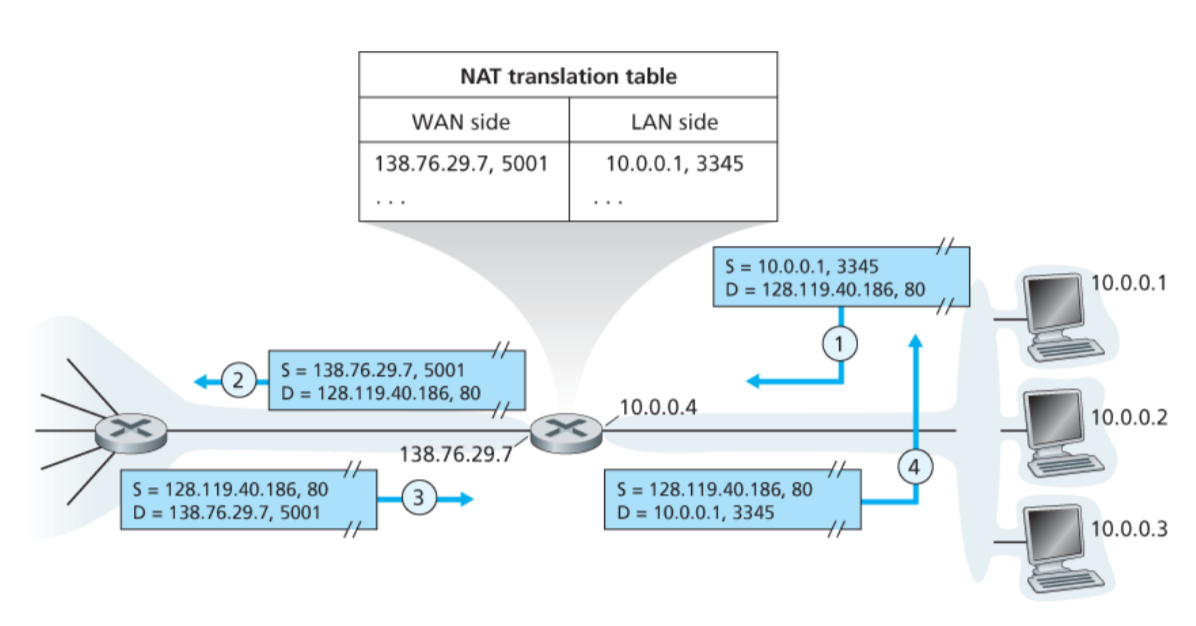
\includegraphics[scale=0.6]{nat.png}
\caption{Network Address Translation}
\label{fig:nat}
\end{figure}

When a host that behinds the NAT want to communicate to the Internet, the NAT-router will translate the host address. Figure~\ref{NAT} shows that how to translate the host address. Suppose a user sitting in a home network behind host 10.0.0.1 requests a Web page on some Web server (port 80) with IP address 128.119.40.186. The host 10.0.0.1 assigns the (arbitrary) source port number 3345 and sends the datagram into the LAN. The NAT router receives the datagram, generates a new source port number 5001 for the datagram, replaces the source IP address with its WAN-side IP address 138.76.29.7, and replaces the original source port number 3345 with the new source port number 5001.

\subsection{IP Datagram Format}

\begin{figure}[h]
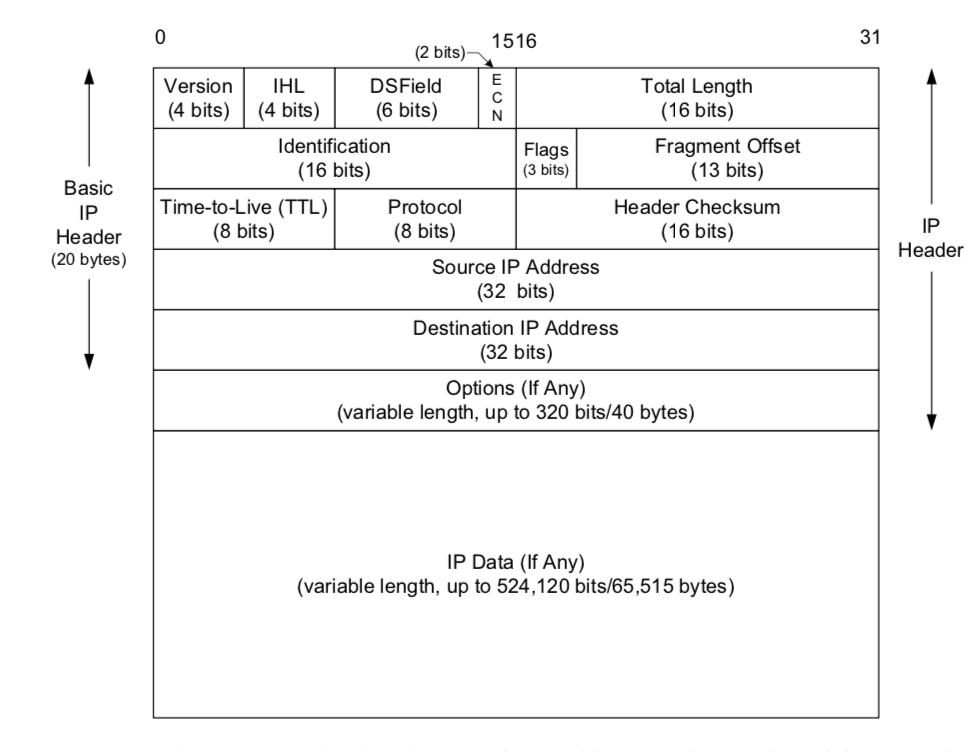
\includegraphics[scale=0.6]{ipv4-datagram-format.png}
\caption{The IPv4 datagram format. A typical IPv4 header contains 20 bytes (no options)}
\label{fig:ipv4-datagram-format}
\end{figure}

The key fields in the IPv4 datagram are the following:\\

\begin{itemize}
\item \textbf{Version} specify the IP protocol version of the datagram (4 or 6).
\item \textbf{IHL - Header Length} is the length of header data.
\item \textbf{Total length} is length of payload data.
\item \textbf{Identification.} The Identification field helps indentify each datagram sent by an IPv4 host.
\item \textbf{TTL.} The Time-to-Live field, or TTL, sets an upper limit on the number of routers through which a datagram can pass.
\item \textbf{Protocol.} The Protocol field in the IPv4 header contains a number indicating the type of data found in the payload portion of the datagram. The most common values are 17 (for UDP) and 6 (for TCP)
\item \textbf{Header Checksum} is calculated over the IPv4 header only to ensure the IP datagram has been correctly delivered.
\item \textbf{Addresses} Every IP datagram contains the Source IP Address of the sender of the datagram and the Destination IP Address of where the datagram is destined. These are 32-bit values for IPv4 and 128-bit values for IPv6. 
\end{itemize}

\subsection{DHCP - Dynamic Host Configuration Protocol}

DHCP allows a host to obtain (be allocated) an IP address automatically. DHCP also allows a host to learn additional information, such as its subnet mask, the address of its first-hop router (often called the default gateway), and the address of its local DNS server (query the IP address from the domain name). DHCP is an Application Layer protocol.\\

DHCP is a client-server protocol. A client is typically a newly arriving host wanting to obtain network configuration information, including an IP address for itself.  Each subnet  will have a DHCP server. If no server is present on the subnet, a DHCP relay agent (typically a router) that knows the address of a DHCP server for that network is needed.\\

\begin{figure}[h]
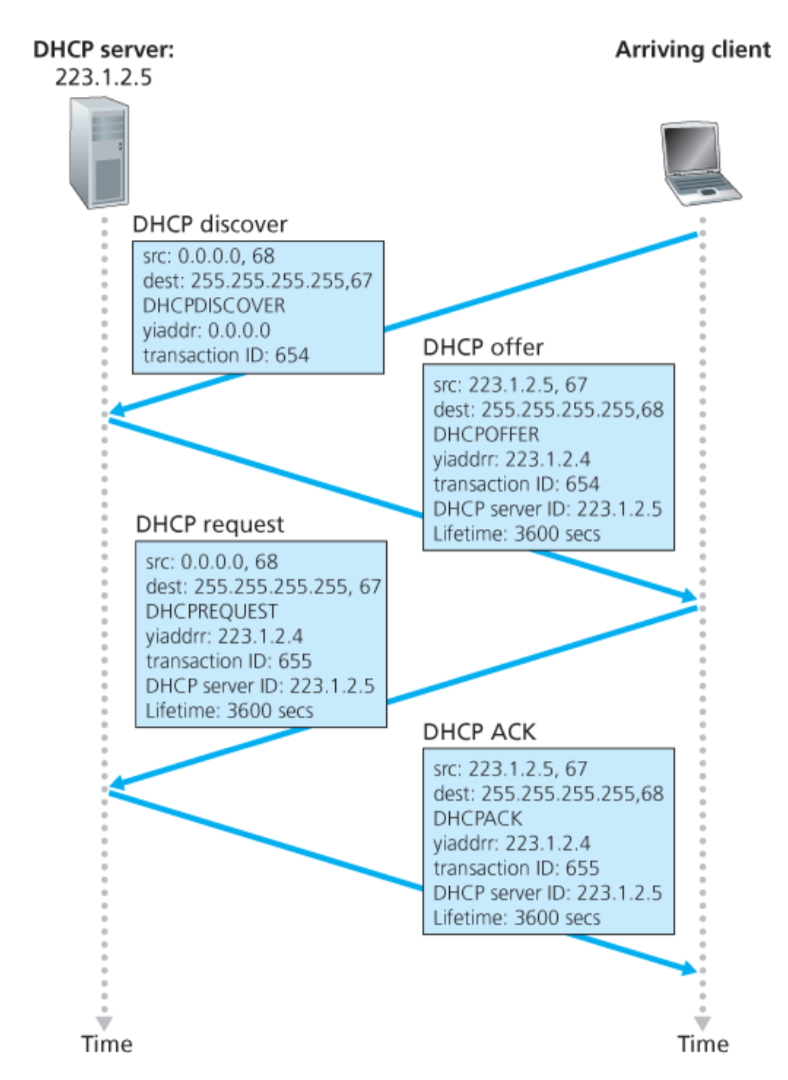
\includegraphics[scale=0.6]{dhcp-protocol.png}
\caption{The DHCP protocol. Client-server interaction}
\end{figure}

When a new client host joining the network, there are four steps to obtain an IP address using the DHCP protocol.\\

\begin{itemize}
\item \textbf{DHCP server discovery.} The first step is finding a DHCP server using a \textit{DHCP discovery message}. The client sends a UDP (a Transport Layer protocol) packet to port 67 with broadcast destination IP address of 255.255.255.255 and a "this host" source IP address of 0.0.0.0. This packet will be broadcast to all nodes attached to the subnet.
\item \textbf{DHCP server offer(s).}. A DHCP server receiving a DHCP discovery message responds to the client with a \textit{DHCP offer message} that is broadcast to all nodes on the subnet, using the IP 255.255.255.255.
\item \textbf{DHCP request.} The client will choose from among one or more server offers and respond to its selected offers with a \textit{DHCP request message}
\item \textbf{DHCP ACK.} The server responds with a \textit{DHCP ACK message} to confirm the request.
\end{itemize}

\clearpage
\section{Network Routing and Management}

\clearpage
\section{Transport Layer}

The transport layer provides communication services directly to the application processes running on different hosts. There are two important transport protocols are UDP (User Datagram Protocol) and TCP (Transmission Control Protocol). They has different characters to support many applications with various properties.\\

\begin{figure}[h]
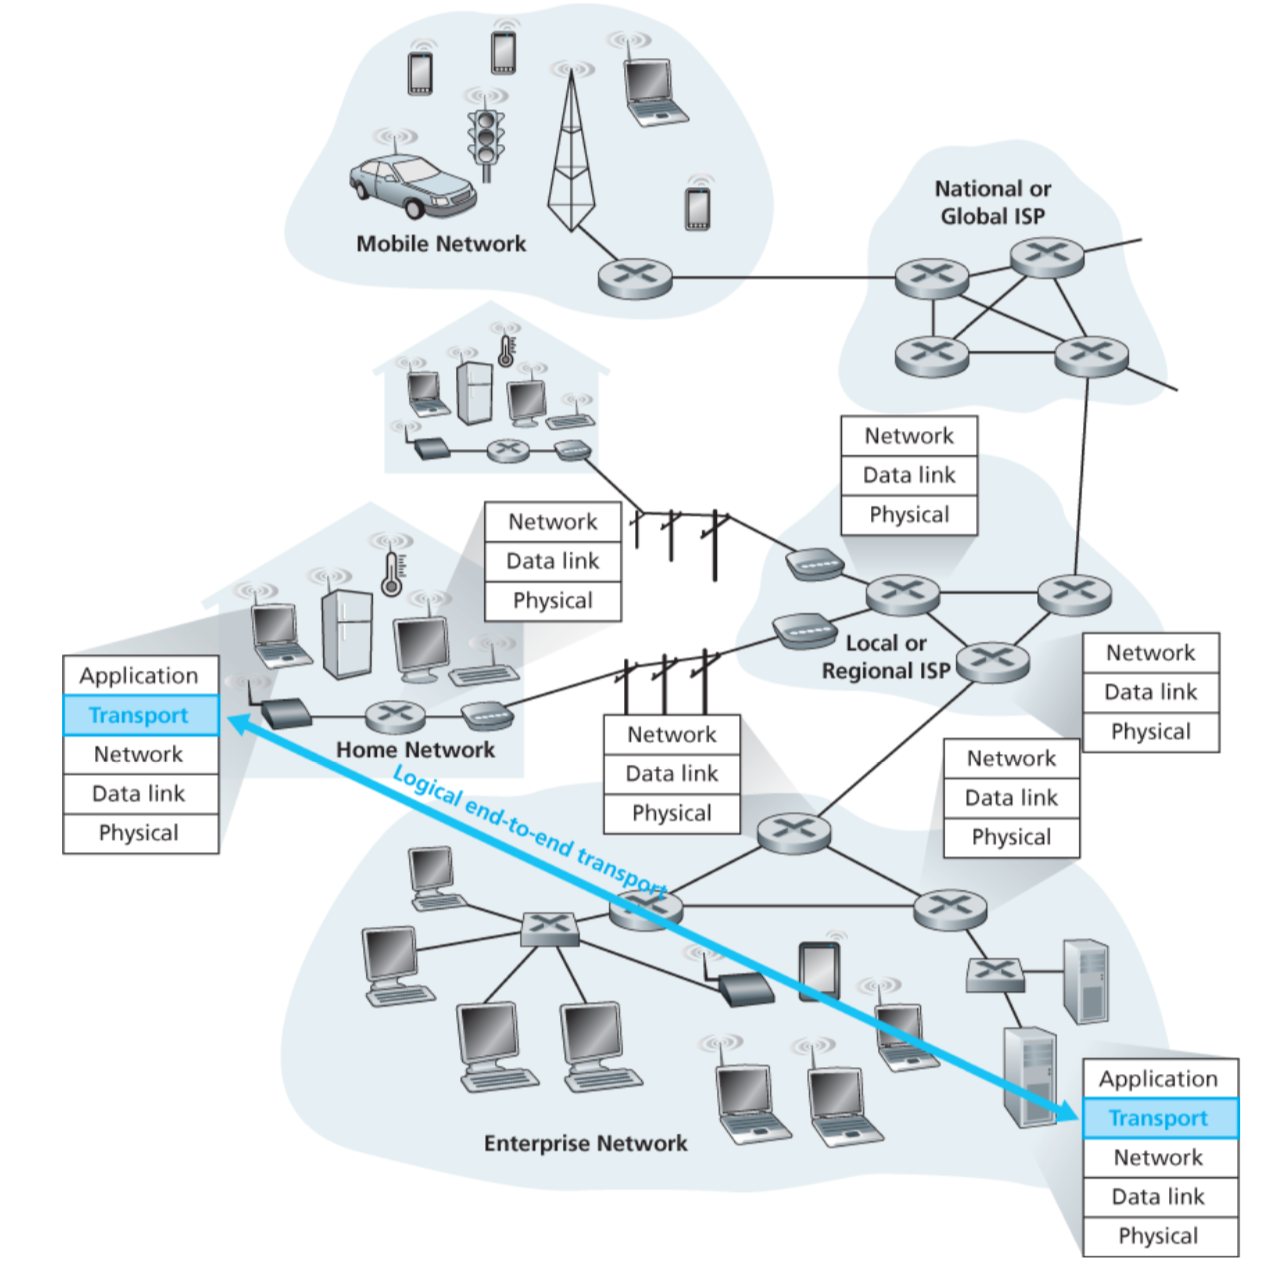
\includegraphics[scale=0.6]{transport-layer.png}
\caption{Transport Layer provides logical rather physical communication between application processes}
\end{figure}

The transport layer protocols are implemented in the host systems but not in network routers. The way, which the transport layer works, can be described as the following steps:\\

\begin{itemize}
\item The transport layer converts the application-messages it receives from a sending application process into \textit{transport-layer segment}. This is done by breaking the application-messages into smaller chunks and adding a transport-layer header to each trunk to create a transport-layer segment. And then
\item Passing each segment to the network layer, where the segment is encapsulated within a network datagram and sent to the destination.
\item At the receiving side, the network layer extracts the transport-layer segment from the datagram and passes the segment up to the transport layer. And then transport layer processes the received segment, making the data in the segment available to the receiving application process.
\end{itemize}

While UDP is the unreliable service, TCP provides \textbf{reliable data transfer}. Using flow control, sequence numbers, acknowledges, and timers, TCP ensures that data is delivered from sending process to receiving process, correctly and in order. Some applications that has a high rate data transmission and can tolerate errors should use the UDP service. Application that needs a reliable communication should use the TCP service.

\subsection{Multiplexing and Demultiplexing} \label{multiplexing}

At the destination host, the transport layer receives segments from the network layer just below. And it has the responsibility to deliver the data of these segments to the appropriate application processes running in the host. Let look an example. You are using your computer with three application processes running: one is downloading a webpage (HTTP process), one is telnet session, and one is downloading a file (FTP process). The transport layer in your computer receives data from the network below, it needs to direct the received data to one of these processes. How this is done?\\

A process can send data to another process on a different host through a door called \textbf{socket}. Sockets are interfaces to use TCP/IP services as communication channels between application processes on networks. A application process can have one or more sockets. Each socket has a unique identifier in the host system called a \textbf{socket port}. A port is a 16-bit number, ranging from 0 to  65535. The port numbers from 0 to 1023 are called \textbf{well-known} ports. They usually are restricted and reserved for well-known application protocols such as HTTP (80), FTP (21), DHCP (67).\\

Each transport segment has two fields: \textbf{source port number} and \textbf{destination port number} in its header. The transport layer will examine these field to identify which socket should direct the segment to. This job is called \textbf{demultiplexing}. The job of gathering data chunks at the source host from different sockets, encapsulating each of them with header to creates segments, and passing these segments to the network layer is called \textbf{multiplexing}.\\

\paragraph{Connectionless Multiplexing and Demultiplexing in UDP}
At a receiving host system, two UDP segments with different source ports but the same destination port will be directed to the same UDP socket. So, an UDP socket is identified by \textit{destination IP address}  and \textit{destination port number}.

\begin{figure}[h]
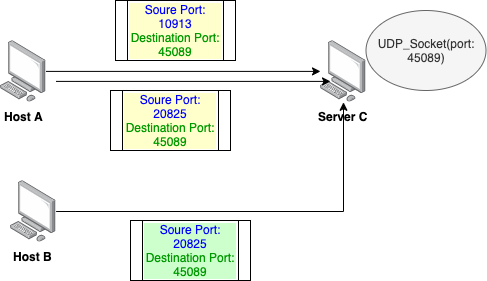
\includegraphics[scale=0.6]{UDP-demultiplexing.png}
\caption{The UDP demultiplexing}
\end{figure}

\paragraph{Connection-Oriented Multiplexing and Demultiplexing in TCP}
A TCP socket is identified by a four-tuple: (source IP address, source port number, destination IP address, and destination port number).At a receiving host stystem, two TCP segments with the same destination port but different source port or different source IP address will be directed to different TCP sockets.

\begin{figure}[h]
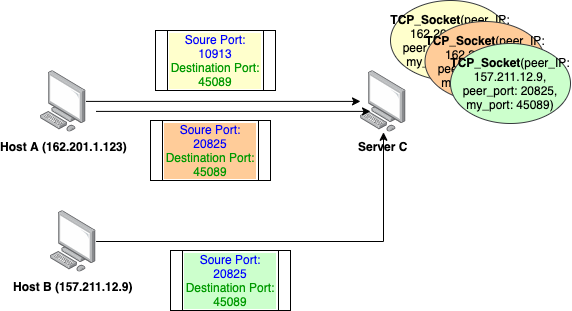
\includegraphics[scale=0.6]{TCP-demultiplexing.png}
\caption{The TCP demultiplexing}
\end{figure}

\subsection{Connectionless Transport: UDP}
The UDP protocol has no connection concept, if a application process want to send a UDP segment, it just pass the segment to the network layer to send to the another process on a different host. The UDP protocol doesn't care about whether the segment is arrived at the receiving side or is it correct. Let look at the UDP segment structure at the figure~\ref{fig:UDP-segment}.

\begin{figure}[h]
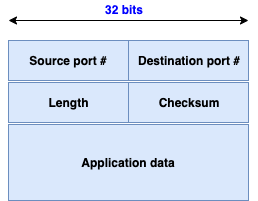
\includegraphics[scale=0.6]{UDP-segment.png}
\caption{The UDP segment structure}
\label{fig:UDP-segment}
\end{figure}

The UDP header has only four fields, each is two bytes. The length field specifies the length in bytes of the UDP header and UDP data. The minimum length is 8 bytes, the length of the header. The field size sets a theoretical limit of 65.535 bytes (8 byte header + 65.527 bytes of data) for a UDP datagram. However to avoid fragmentation in the IP layer, the actual limit for the data length, which is imposed by the underlying IPv4 protocol, is 65.507 bytes (65.535 - 8 byte UDP header - 20 byte IP header). The UDP checksum provides for error detection. The receiving side will use the checksum to determine whether the segment is altered or not.\\

\paragraph{Socket programming with UDP}
Let take a socket programming example to demonstrate how UDP protocol work.\\

We’ll use the following simple client-server application to demonstrate socket programming for both UDP and TCP:

\begin{enumerate}
\item The client reads a line of characters (data) from its keyboard and sends the data to the server. 
\item The server receives the data and converts the characters to uppercase.
\item The server sends the modified data to the client.
\item The client receives the modified data and displays the line on its screen.
\end{enumerate}

\begin{lstlisting}[language=Python, caption= UDP Server]
# Server side
import socket as s

serverSocket = s.socket(s.AF_INET, s.SOCK_DGRAM) # For UDP
serverSocket.bind(('', 12345))

while True:
    message, clientAddress = serverSocket.recvfrom(2048)
    modifiedMessage = message.decode().upper()
    print('Received Messages: {}, from {}'.format(message, clientAddress))
    serverSocket.sendto(modifiedMessage.encode(), clientAddress)
\end{lstlisting}

\begin{lstlisting}[language=Python, caption= UDP Client]
# Client side
import socket as s

serverIP = '127.0.0.1'
serverPort = 12345

clientSocket = s.socket(s.AF_INET, s.SOCK_DGRAM)
message = raw_input('Input lowercase sentence:')
clientSocket.sendto(message.encode(),(serverIP, serverPort))
modifiedMessage, serverAddress = clientSocket.recvfrom(2048)
print(modifiedMessage.decode())
clientSocket.close()
\end{lstlisting}

Server needs to associate to a specific port that is known by clients by using \textbf{bind} method. The \textit{socket} library in Python will call the underline system calls (operating system call). You can learn more about Socket API in C by referencing \url{https://en.wikipedia.org/wiki/Berkeley_sockets}

\subsection{Connection-Oriented Transport: TCP}

TCP provides reliability, error recovery and  flow control. TCP protocol is a connection-oriented protocol. Two processes will communicate to each other over a TCP connection. The figure~\ref{fig:tcp-connection-oriented} shows a logical TCP connection between two processes.

\begin{figure}[h]
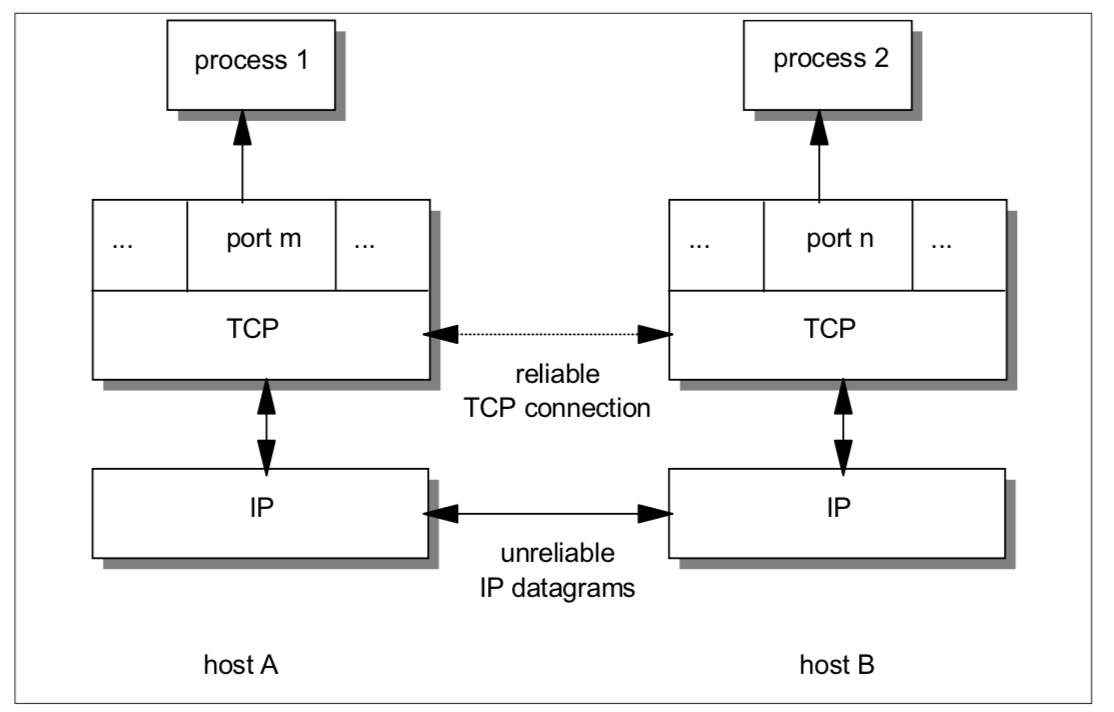
\includegraphics[scale=0.6]{tcp-connection.png}
\caption{TCP: Connection between processes}
\label{fig:tcp-connection-oriented}
\end{figure}

TCP can provide the following facilities to applications:

\begin{itemize}
\item \textit{Stream data transfer}: From the application's point of view, TCP transfers a contiguous stream of bytes through the network. TCP does this by grouping the bytes into TCP segments, which are passed to the IP layer for transmission to the destination.
\item \textit{Reliability}: TCP assigns a sequence number to each segment transmitted, and expects an acknowledge (ACK) from the receiving TCP layer. If the ACK is not received within a timeout interval, the segment is re-transmitted. And the receiving side uses the sequence numbers to rearrange the segments where they arrive out of order, and eliminates the duplicate segments.
\item \textit{Flow control}: The receiving TCP, when sending an ACK back to the sender, also indicates to the sender the number of bytes it can receive (without overun and overflow in it internal buffer). This mechanism is referred to the window-mechanism, and we discuss it later.
\item \textit{Multiplexing and Demultiplexing}: Refer to section \ref{multiplexing}
\item \textit{Logical connections}: The reliability and flow control mechanisms described here require that TCP initializes and maintains certain status information for each data stream. The combination of this status, including sockets, sequence numbers, and window sizes, is called a logical connection. Each connection is identified by the pair of sockets used by the sending and receiving processes.
\item \textit{Full duplex}: TCP supports concurrent data streams in both directions.
\end{itemize}

\subsubsection{The window-principle}
To achieve the reliability, TCP can transmit a segment and wait the ACK. When the ACK received, TCP then transmits the next segment. But this solution wastes the network bandwidth. An other solution is sending and waiting ACK of a group of segments called a window. Let take an example where window size is 5. At the first, TCP can send 5 segments without waiting for any ACK. 

\begin{figure}[h]
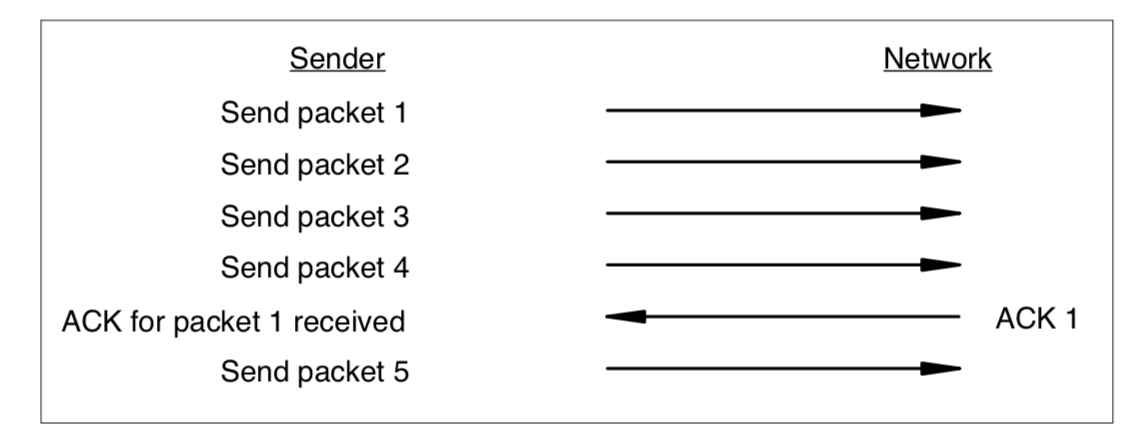
\includegraphics[scale=0.6]{window-principle.png}
\caption{TCP: Window principle}
\label{fig:window-principle}
\end{figure}

As shown in the figure~\ref{fig:window-principle}, at the moment the sender receives ACK 1 (ACK n has next expect sequence number is n + 1 - means that the receiver has receive segment n in sequenced and expects the next segment n + 1), it can slide its window one segment to the right. The window now contains segment 2 to 6, TCP can sent segment 6. Let look some other scenarios:

\begin{itemize}
\item Packet 2 gets lost: The sender will not receive ACK 2. It received and acknowledged segment 3, 4, 5 with ACK 1, because segment 1 was the last one received in sequence. After timeout, the sender will re-transmit segment 2. If receiver received segment 2, it will acknowledge with ACK 5. And if ACK 5 was arrived at the sender, the window will slice four positions.
\item Packet 2 did arrive, but the acknowledge gets lost: The sender doesn't receive ACK 2, but will receive ACK 3. ACK 3 is an acknowledge for all segments up to 3 and now the sender slide its window to packet 4.
\end{itemize}

\begin{figure}
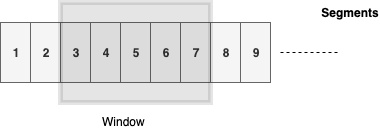
\includegraphics[scale=0.6]{window-slice.png}
\caption{Window slice: segment 2 is the last one receive in sequence, segment 3 is not acknowledged}
\label{fig:window-slice}
\end{figure}

\subsubsection{The TCP segment format}

\begin{figure}[h]
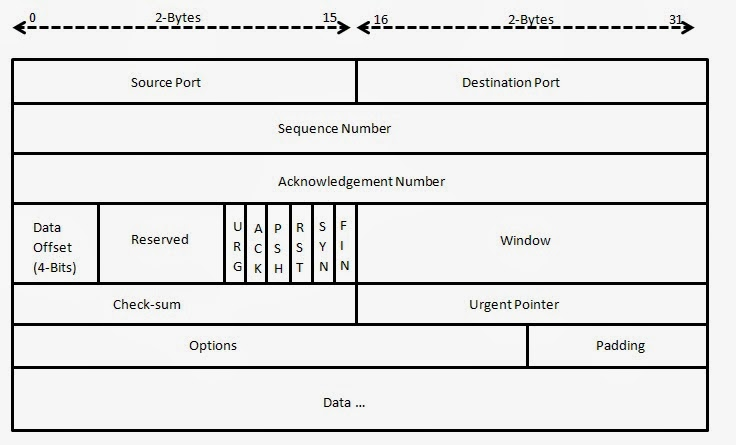
\includegraphics[scale=0.6]{tcp-segment-format.jpg}
\caption{The TCP segment format}
\label{fig:tcp-segment-format}
\end{figure}

Figure~\ref{fig:tcp-segment-format} shows the format of a TCP segment, where:

\begin{itemize}
\item \textbf{Source port.} The 16-bit source port number. Used by the receiver to reply.
\item \textbf{Destination port.} The destination port number.
\item \textbf{Sequence number.} In fact, this field is the sequence number of the first byte in the segment rather the segment. If the SYN control bit is set, the sequence number is the initial sequence number (ISN) and the first data byte is ISN+1
\item \textbf{Acknowledge number.} If the ACK control bit is set this field contains the value of the next sequence number the sender of the segment is expecting to receive.  Once a connection is established this is always sent.
\item \textbf{Data offset.} 4 bits field indicates where the data begins.
\item \textbf{Reserved.} 6 bits field is reserved for future use. Must be zero.
\item \textbf{Control bits.} 6 bits, from left to the right
   \begin{itemize}
    \item URG:  Urgent Pointer field significant
    \item ACK:  Acknowledgment field significant
    \item PSH:  Push Function
    \item RST:  Reset the connection
    \item SYN:  Synchronize sequence numbers
    \item FIN:  No more data from sender
   \end{itemize}
\item \textbf{Window.} Window size (in bytes)
\item \textbf{Checksum.} The checksum of header and data
\end{itemize}

\subsubsection{Acknowledgments and Re-transmissions}
TCP sends data in variable length of segments. Sequence numbers are based on a byte count. Acknowledgments specify the sequence number of the next byte that the receiver expects to receive. Figure~\ref{fig:ack-retransmit} shows an example of acknowledgment and retransmission. Assume that the window size is 1500 bytes and segment size is 500 bytes.

\begin{figure}[h]
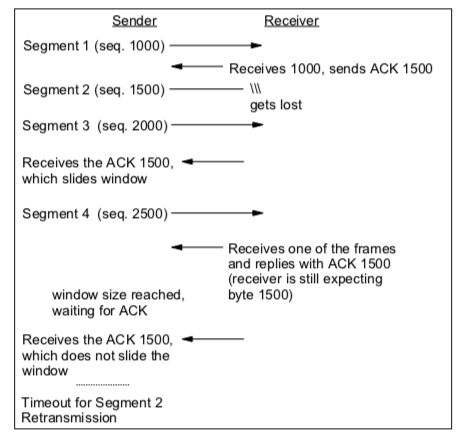
\includegraphics[scale=0.6]{ack-and-retransmit.png}
\caption{The acknowledgments and re-transmissions}
\label{fig:ack-retransmit}
\end{figure}

\subsubsection{TCP Connection Management}
Before exchanging any data, a connection has to be established between two application processes. One process acts as a listening side (inactive side or server) and other acts as a initiating side (active side or client). The server listens a connection from a client. As shown in Figure~\ref{fig:tcp-connection-establish}, a connection is established in three steps.

\begin{figure}[h]
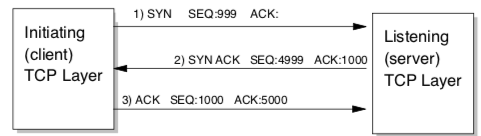
\includegraphics[scale=0.6]{tcp-connection-establish.png}
\caption{TCP connection establishment}
\label{fig:tcp-connection-establish}
\end{figure}

\begin{itemize}
\item \textbf{Step 1 (SYN)}:  In the first step, client wants to establish a connection with server, so it sends a segment with SYN(Synchronize Sequence Number) and set the sequence number is usually a random value called N.
\item \textbf{Step 2 (SYN+ACK)}: Server responds to the client with SYN-ACK bits set. The acknowledgement number is set to one more then the received sequence number N+1, and the sequence number that the server chooses for the packet is another random number, M.
\item \textbf{Step 3 (ACK)}: Finally, the client sends an ACK back to the server. The sequence number is set to the received acknowledgement value N+1, and the acknowledgement number is set to one more than the received sequence number M+1
\end{itemize}

Closing the connection is done implicitly by sending a FIN segment (no more data). Because the connection is full-duplex, the FIN segment only closes the data transfer in one direction, the whole process is represented in the figure~\ref{fig:tcp-close}. 

\begin{figure}[h]
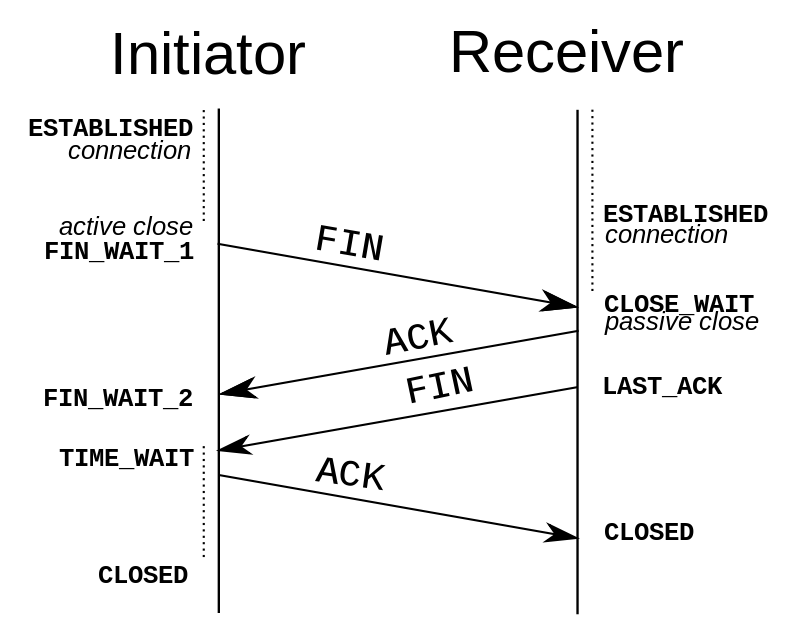
\includegraphics[scale=0.3]{tcp-close.png}
\caption{Connection termination}
\label{fig:tcp-close}
\end{figure}

The following is a list of the different states of a TCP connection:

\begin{itemize}
\item LISTEN - represents waiting for a connection request from any remote TCP and port.
\item SYN-SENT - represents waiting for a matching connection request after having sent a connection request.
\item SYN-RECEIVED - represents waiting for a confirming connection request acknowledgment after having both received and sent a connection request.
\item ESTABLISHED - represents an open connection, data received can be delivered to the user.  The normal state for the data transfer phase of the connection.
\item FIN-WAIT-1 - represents waiting for a connection termination request from the remote TCP, or an acknowledgment of the connection termination request previously sent.
\item FIN-WAIT-2 - represents waiting for a connection termination request from the remote TCP.
\item CLOSE-WAIT - represents waiting for a connection termination request from the local user.
\item CLOSING - represents waiting for a connection termination request acknowledgment from the remote TCP.
\item LAST-ACK - represents waiting for an acknowledgment of the connection termination request previously sent to the remote TCP (which includes an acknowledgment of its connection termination request).
\item TIME-WAIT - represents waiting for enough time to pass to be sure the remote TCP received the acknowledgment of its connection termination request.
\item CLOSED - represents no connection state at all.
\end{itemize}

\subsubsection{Programming Interface: Socket API}
The Socket Interface is a network communication API, it was first introduced in the 4.2BSD UNIX-base system. Socket APIs provide the following actions:
\begin{itemize}
\item Initialize a socket
\item Bind (register) a socket to an address (port and address)
\item Listen on a socket for  connections
\item Accept a connection
\item Connect to a server
\item Send and receive data on a socket
\item Close a socket
\end{itemize}

The base standard of socket APIs known as BSD socket API. The core functions of this standard are:\\

\noindent Initialize a socket: \textit{socket(domain, type, protocol): int} return a file descriptor\\
 	\begin{tabular}{ p{2cm} p{10cm} }
 		\textbf{domain} & This determines the communication protocol: AF\_INET (IPv4 Internet domain), AF\_INET6 (IPv6 Internet domain), AF\_UNIX (UNIX domain)\\
 		\textbf{type} & This is type of socket: SOCK\_DGRAM (for UDP socket), SOCK\_STREAM (for TCP socket), SOCK\_RAW (datagram interface to IP)\\
 		\textbf{protocol} & The protocol specifies a particular protocol to be used with the socket. Normally only a single protocol exists to support a particular socket type within a given protocol family. Leave it 0 if you don't care.
 	\end{tabular}
 	
\noindent Bind a socket to an address: \textit{bind(sockfd, addr, addrlen)}\\
	\begin{tabular}{ p{2cm} p{10cm} }
 		\textbf{sockfd} & The socket fd to bound. This value was create in the previous function\\
 		\textbf{addr} & This is a pointer to a protocol-specific address\\
 		\textbf{addrlen} & This is the size of the address structure.
 	\end{tabular}
 	
\noindent Listen on a socket for inbound connections: \textit{listen(sockfd, backlog)}\\
	\begin{tabular}{ p{2cm} p{10cm} }
		\textbf{sockfd} & The socket fd to listen on\\
		\textbf{backlog} & The backlog parameter defines the maximum length for the queue of pending connections
	\end{tabular}
	
\noindent Establish a connection with a TCP server: \textit{connect(sockfd, serveraddr, addrlen)}\\
	\begin{tabular}{ p{2cm} p{10cm} }
		\textbf{sockfd} & The socket fd used to connect the server\\
		\textbf{serveraddr} & The pointer to the server address structure\\
		\textbf{addrlen} & The size of the address structure
	\end{tabular}

\noindent Send data on a socket:\textit{send(sockfd, buffer, len, flags)}\\
	\begin{tabular}{ p{2cm} p{10cm} }
		\textbf{sockfd} & The socket fd used to send data\\
		\textbf{buffer} & The buffer contains data\\
		\textbf{len} & The size of data\\
		\textbf{flags} & This is an option: MSG\_OOB out of band, MSG\_DONTROUTE bypass routing, use direct interface
	\end{tabular}

\noindent Receive data from a socket: \textit{recv(sockfd, buffer, len, flags)}\\
	\begin{tabular}{ p{2cm} p{10cm} }
		\textbf{sockfd} & The socket fd used to receive data\\
		\textbf{buffer} & The buffer to  receive data\\
		\textbf{len} & The size of data received\\
		\textbf{flags} & This is an option: MSG\_OOB out of band, MSG\_PEEK peek at incoming message, MSG\_WAITALL wait for full request or error
	\end{tabular}
\noindent Close a socket: \textit{close(sockfd)}\\

\begin{figure}[h]
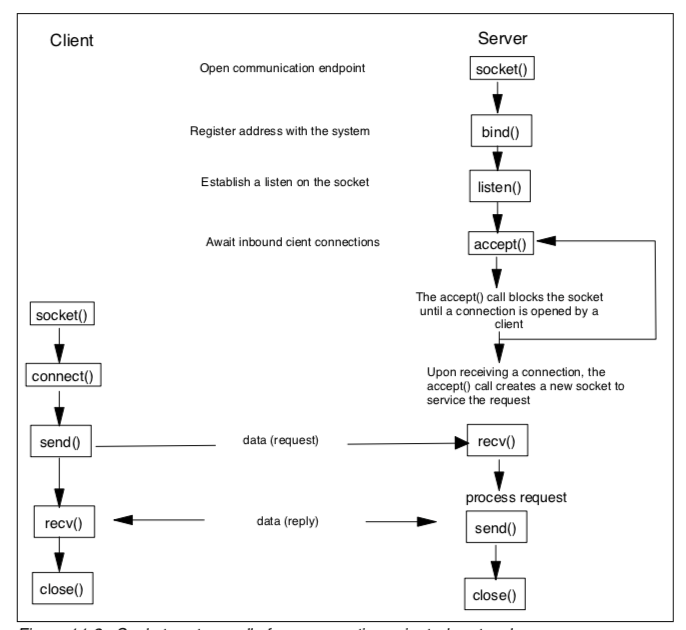
\includegraphics[scale=0.6]{client-server-socket.png}
\caption{Client/server communication model with socket}
\label{fig:client-server-socket}
\end{figure}

Figure~\ref{fig:client-server-socket} show an example of a client/server communication.

\clearpage
\section{Application Layer}
The network provides services to build distributed applications called network applications. Network application use the transport services TCP or UDP to transfer data (often called messages) between application processes. Applications define the structure of messages and when to send they. These definition establish application protocols:
\begin{itemize}
\item The type and structure of messages
\item The semantics of message's fields
\item When and how a process sends messages and responds to messages
\end{itemize}

\begin{figure}[h]
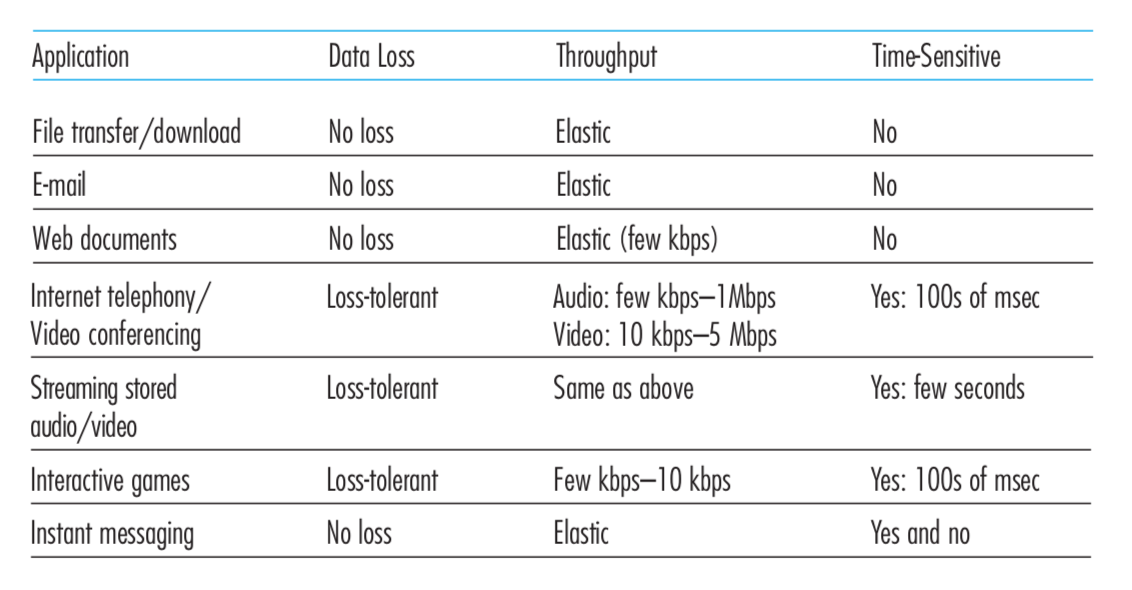
\includegraphics[scale=0.6]{application-requirement.png}
\caption{Requirements of network applications}
\label{fig:application-requirement}
\end{figure}

\begin{figure}[h]
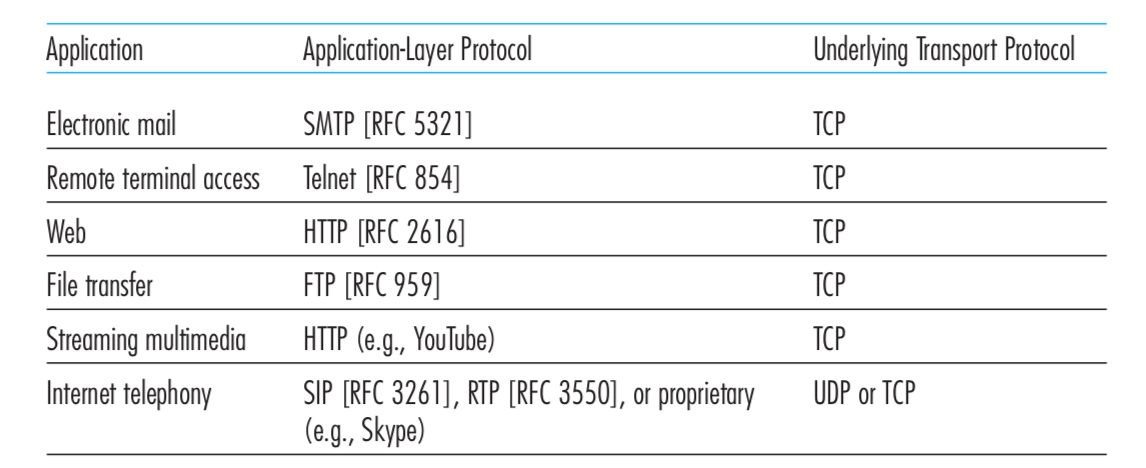
\includegraphics[scale=0.6]{application-protocols.png}
\caption{Application protocols and their underlying transport protocols}
\label{fig:application-protocol}
\end{figure}

Different applications have different characters and requirements, and then we will use either TCP or UDP services for these applications. Figure~\ref{fig:application-requirement} shows the service requirements of some network applications. Depend on these requirements, application protocols will use different underlying transport protocols as shown in figure~\ref{fig:application-protocol}.

\subsection{The Web and HTTP Protocol}
Web is a network application that contains web servers and web clients. Clients request resources from servers. They talk to each other using a application protocol called HTTP (Hypertext Transfer Protocol). Clients are web browsers like Firefox, Chrome, or any other HTTP client. In early of Web, resources, which are served by web servers, are Web pages (is a HTML page that has some links to other websites - public addresses of web servers). But today, web resources can be anything such as image, audio, video files each of that is addressable by a single URL. An URL has the form:

\[<protocol>://<domain>/<path-to-resource>\]
For example, the URL

\[http://www.someCollege.com/someDepartment/picture.jpg\]
has \textit{http} is the protocol, \textit{www.someCollege.com} is the domain and \textit{someDepartment/picture.jpg} is the path of resource.\\

HTTP defines how Web clients request resources from Web servers and how servers transfer resources to clients. HTTP uses TCP as its underlying transport protocol. Each request and response can be made over a \textit{seperate} TCP connection, which called \textbf{non-persistent connection}. TCP is designed to transfer a stream of data, but HTTP requests and responses often are short time. Using non-persistent connection causes many TCP connections are created and closed that waste much time. Hence, HTTP uses \textbf{persistent connections} that means many request/response pairs are took care by a TCP connection, and a timeout interval used to end the TCP connection.\\

\subsubsection{HTTP Message Format}
There are two types of HTTP messages, request messages and response messages.\\
\textbf{HTTP Request Format}\\
Let see a typical HTTP request message:\\
{\ttfamily
GET /somedir/page.html HTTP/1.1 \\
Host: www.somesite.edu \\
User-agent: Mozilla/5.0 \\
Accept-language: en} \\

The first line is called the \textbf{request line}, and the subsequent lines are called the \textbf{header lines}. The request line has three fields: the method field, the URL field, and the HTTP version field. The method field can take on several different values, including GET, POST, HEAD, PUT,and DELETE. The great majority of HTTP request messages use the GET method. The GET method is used when the browser requests an object, with the requested object identified in the URL field. Figure~\ref{fig:http-request-format} shows the general format of an HTTP request message.

\begin{figure}[h]
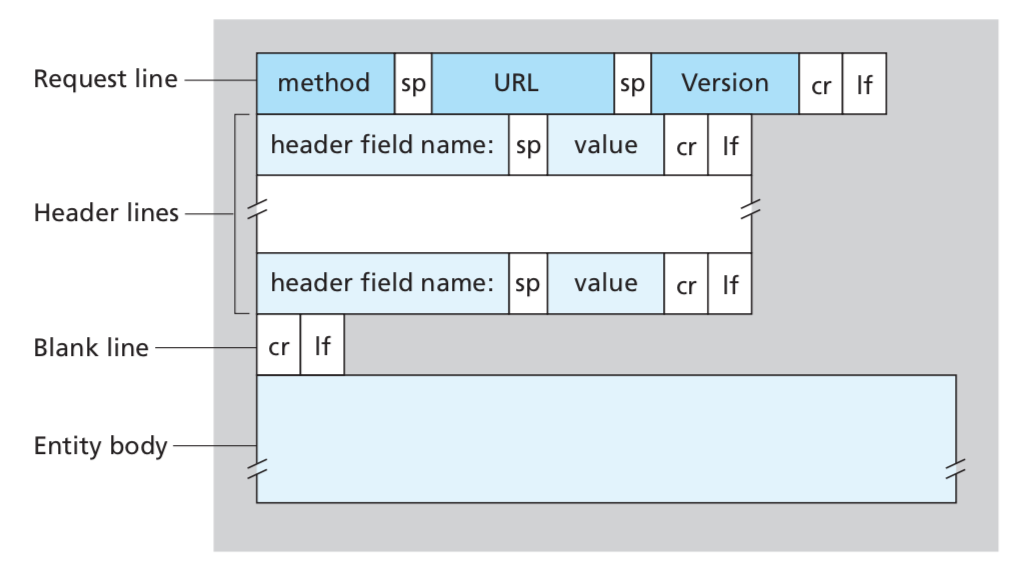
\includegraphics[scale=0.7]{http-request-format.png}
\caption{The format of an HTTP request message}
\label{fig:http-request-format}
\end{figure}

\noindent \textbf{HTTP Response Format}\\
Let see a typical HTTP response message:\\
{\ttfamily
HTTP/1.1 200 OK\\
Date: Mon, 23 May 2011 22:38:34 GMT\\
Content-Type: text/html; charset=UTF-8\\
Content-Length: 155\\
Last-Modified: Wed, 08 Jan 2011 23:11:55 GMT\\
Server: Apache/1.3.3.7 (Unix) (Red-Hat/Linux)\\
Connection: close\\

\noindent (data data data data data ...)}\\

The response has three sections: an initial status line, header lines, and then the entity body. The entity body contains the requested object itself (represented by data data data data data ...). The status line has three fields: the protocol version field, a status code, and a corresponding status message. The general format of an HTTP response is shown as figure~\ref{fig:http-response-format}.

\begin{figure}[h]
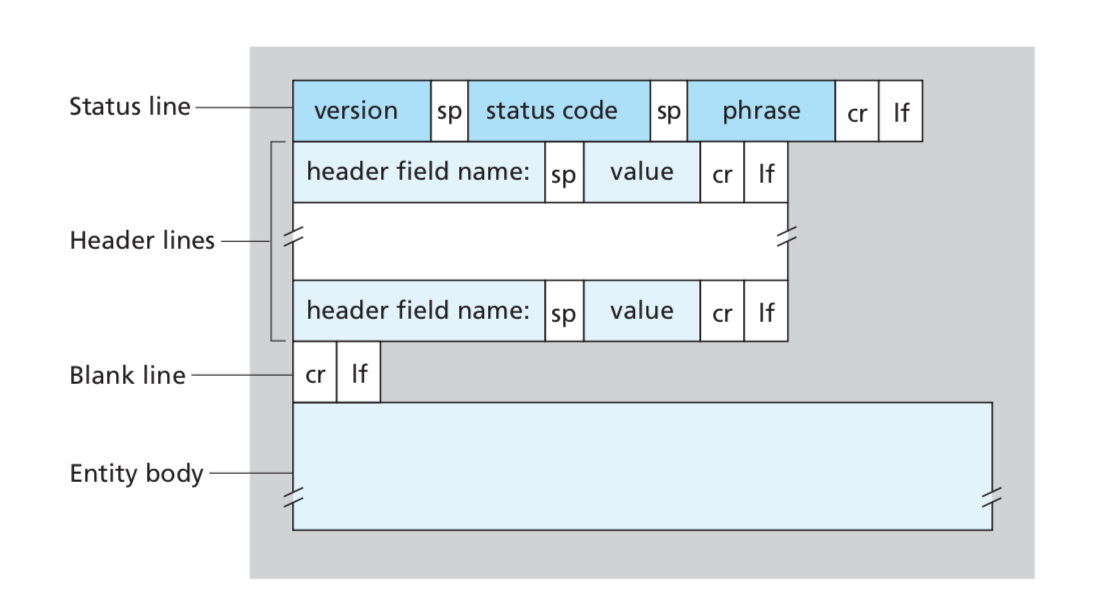
\includegraphics[scale=0.7]{http-response-format.png}
\caption{The format of an HTTP response message}
\label{fig:http-response-format}
\end{figure}

\subsection{Electronic Mail - Email}
Email is an asynchronous communication medium - you send and read messages when it is convenient for you. Modern email has many features, including messages with attachments, hyperlinks, HTML embedded, and images embedded. Figure~\ref{fig:email-system} shows a high-level view of the Internet email system. The diagram has three major components: \textbf{user agents}, \textbf{mail services}, and the \textbf{Simple Mail Transfer Protocol (SMTP)}.\\

\begin{figure}[h]
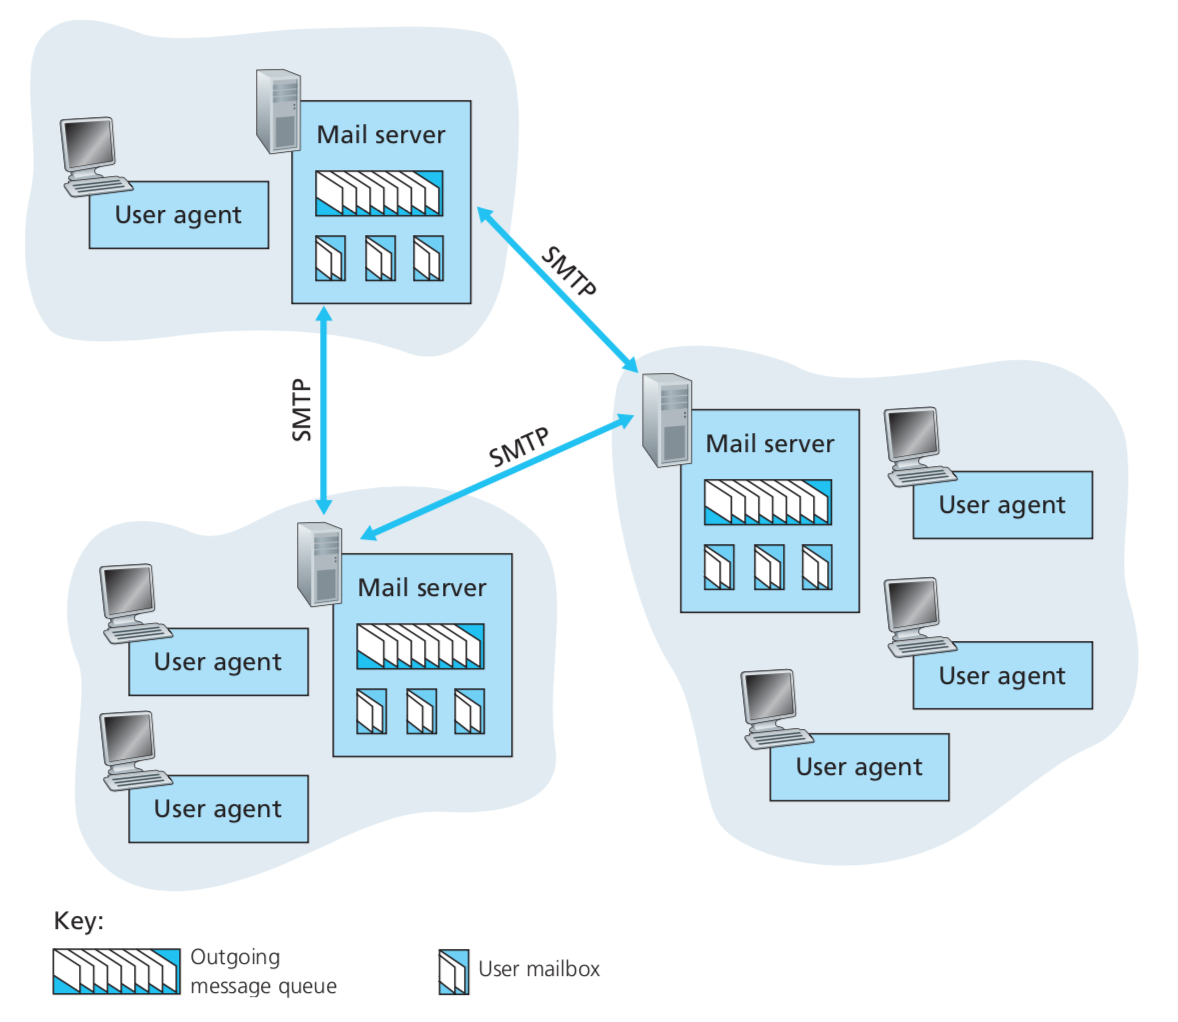
\includegraphics[scale=0.6]{email-system.png}
\caption{A high-level view of the Internet email system}
\label{fig:email-system}
\end{figure}

Users can use user agents to read, reply, forward, save and compose messages. Microsoft Outlook, Thunderbolt, and Apple Mail are examples of user agents for email. Alice uses her user agent to compose a message (an email), and then her agent sends the email to the Alice's mail server. The Alice's mail server will send (\textit{relay}) the email to the Bob's mail server. The Bob's mail server places the email into his mail-box. Each user will have a mail-box located in his mail-server. Bob uses an user agent to read the email from his mail-box on the mail-server. If the Alice's mail-server cannot delivery mail to the Bob's mail-server, it holds the message in a \textbf{message queue} and attempts to transfer the message later. That is why Alice's user agent doesn't send mail direct to the Bob's mail-server.\\

Alice's user agent sends mail to the Alice's mail-server and the Alice's mail-server sends mail to the Bob's mail-server using the SMTP protocol - a push protocol. Bob's user agent uses a pull protocol to pull mails from Bob's mail-server. POP3, IMAP, and HTTP are popular pull protocol used to pull mails from server. Figure~\ref{fig:email-protocol} summarizes the protocols that are used for the Internet email.\\

\begin{figure}[h]
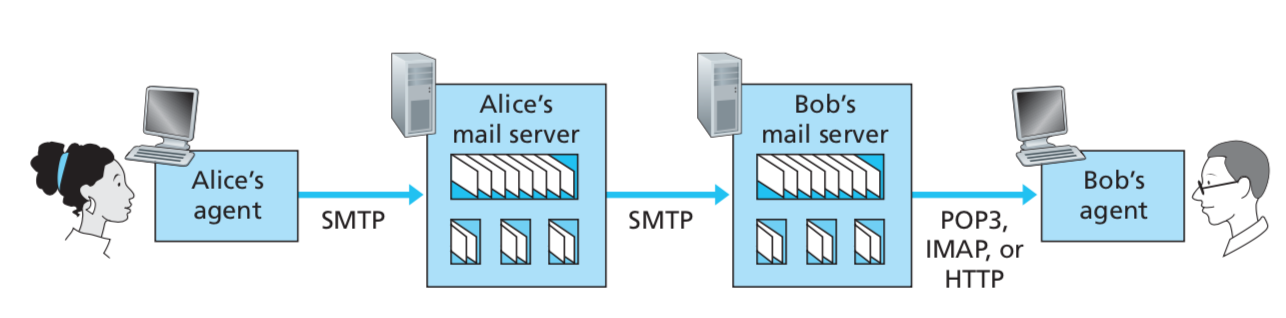
\includegraphics[scale=0.6]{email-protocol.png}
\caption{Email flow and protocols}
\label{fig:email-protocol}
\end{figure}

A email contains header and body that are separated by a blank line. A message header looks like this:\\
{\ttfamily
From: alice@crepes.fr\\
To: bob@hamburger.edu\\
Subject: The networking conference invitation.}\\

\subsection{Domain Name System - DNS}
To communicate to a host in the Internet, you need to remember its IP address. But as human, it is difficult to remember a dotted-decimal IP address. So, \textbf{hostnames} is used as a readable identification solution to hosts in the Internet. Examples of hostnames are \textit{www.yahoo.com}, \textit{ocw.mit.edu} that are therefore appreciated by humans.\\

The main task of the Internet's \textbf{domain name system (DNS)} is translating hostnames to IP addresses. When an application need to translate a hostname to an IP address, it send a DNS request to a \textbf{DNS Server} and the server will respond by a DNS reply. All DNS requests and replies are send within UDP datagrams to port 53. To avoid the single point of failure and traffic volume and deal with issue of scale, DNS servers are organized in a hierarchical structure and distribute around the world as shown in figure~\ref{fig:dns-hierarchy}.\\

\begin{figure}[h]
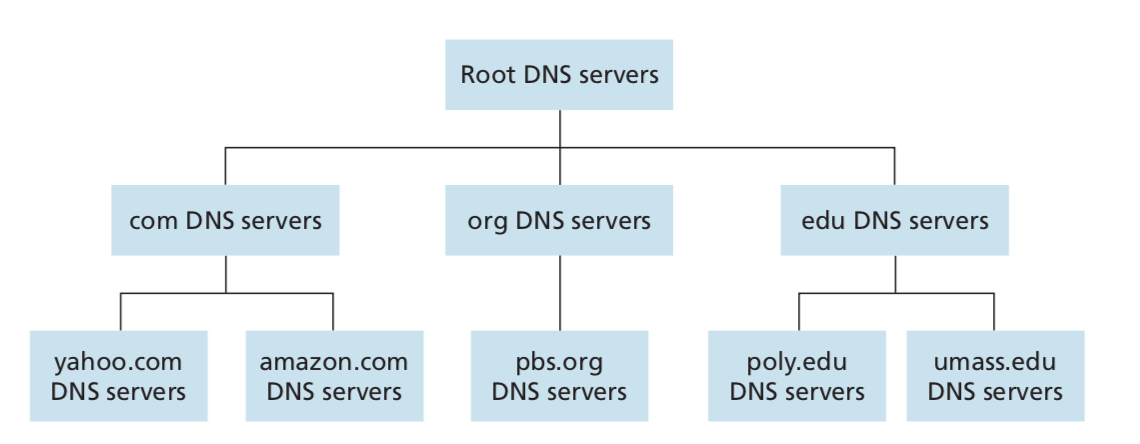
\includegraphics[scale=0.6]{dns-hierarchical-organization.png}
\caption{The hierarchy of DNS servers}
\label{fig:dns-hierarchy}
\end{figure}

\end{document}